\documentclass[11pt,a4paper]{article}

% --- Packages ---
\usepackage[margin=1in]{geometry}
\usepackage{graphicx}
\usepackage{amsmath,amssymb}
\usepackage{booktabs}
\usepackage{hyperref}
\usepackage{xcolor}
\usepackage{float}
\usepackage{caption}
\usepackage{natbib}
\usepackage{enumitem}
\usepackage{longtable}
\usepackage{multirow}

\hypersetup{
    colorlinks=true,
    linkcolor=blue!60!black,
    citecolor=blue!60!black,
    urlcolor=blue!60!black
}

\graphicspath{{figures/}}

\title{\textbf{Seasonal Salinity as a Latitude-Dependent\\Disease Suppression Mechanism\\in the SSWD-EvoEpi Model}}
\author{Anton Starkov}
\date{March 13, 2026}

\begin{document}

\maketitle

% ============================================================
\section{Executive Summary}
% ============================================================

This report documents the design, predictions, and validation of a seasonal salinity mechanism introduced into the SSWD-EvoEpi model. The mechanism addresses a longstanding calibration challenge: the observed north--south gradient in Sea Star Wasting Disease (SSWD) dynamics across the 896-node coastal network spanning Alaska ($\sim$61\textdegree N) to Baja California ($\sim$30\textdegree N).

The core insight is that glacial and snowmelt-driven freshwater pulses depress nearshore salinity at high-latitude, fjord-dominated sites during summer months, creating conditions unfavorable for \textit{Vibrio}-mediated disease transmission. This effect is strongest in enclosed fjords (high \texttt{fjord\_depth\_norm}) at high latitudes, and essentially absent along exposed California coastline.

\textbf{Key findings:}
\begin{itemize}[nosep]
    \item The model introduces two new calibration parameters: \texttt{fw\_strength} (range 6--25 psu) and \texttt{fw\_depth\_exp} (range 0.3--3.0).
    \item At \texttt{fw\_strength}~=~15, mean June salinity depression reaches 12.76~psu in AK-FN (95\% of nodes with $\texttt{fd\_norm} > 0.5$), while California regions experience $<$0.4~psu depression.
    \item The Alaska--California asymmetry in Vibrio suppression is total: 35.01\% mean June suppression in Alaska vs.\ 0.0\% in California.
    \item Validation against 8 DFO lighthouse stations in British Columbia shows the model captures the qualitative seasonal cycle (1.6--6.0 psu observed ranges) despite systematic positive bias in the ocean baseline.
    \item The mechanism is backward-compatible: setting \texttt{fw\_strength}~=~0 recovers the original constant-salinity model.
    \item Peak salinity depression of 15.0 psu occurs at node AK-PWS-002 (61.11\textdegree N, $\texttt{fd\_norm} = 1.0$).
\end{itemize}

The report presents the observational basis, model equations, spatial predictions across all 18 regions, sensitivity analyses, DFO validation, and implications for ongoing MCMC calibration.

% ============================================================
\section{Motivation: The Latitude Gradient Problem}
\label{sec:motivation}
% ============================================================

The SSWD-EvoEpi model simulates disease dynamics across 896 coastal sites from Alaska to Baja California. A persistent challenge in calibration has been the observed latitudinal asymmetry in disease timing and severity. High-latitude Alaskan sites (275 nodes) experience delayed and sometimes attenuated disease outbreaks relative to lower-latitude California and Oregon sites (238 and 59 nodes, respectively), despite comparable sea star population densities.

One candidate mechanism for this pattern is seasonal freshwater influence on nearshore salinity. \textit{Vibrio} spp., implicated as secondary pathogens or environmental stressors in SSWD, are strongly salinity-dependent. At low salinities, \textit{Vibrio} growth and virulence are suppressed, potentially reducing disease transmission. In the Pacific Northwest and Alaska, massive glacial and snowmelt pulses deliver fresh water to coastal fjords during late spring and summer---precisely the period when warming temperatures would otherwise favor pathogen proliferation.

This creates a natural experiment: enclosed fjord sites at high latitudes experience dramatic seasonal salinity depression, while exposed coastal sites at lower latitudes do not. The question is whether this freshwater effect is large enough to materially alter disease dynamics in the model.

% ============================================================
\section{Observational Basis}
\label{sec:observations}
% ============================================================

\subsection{DFO Lighthouse Climatology}

The primary observational dataset comes from the Department of Fisheries and Oceans (DFO) Canada lighthouse monitoring program. Eight stations along the British Columbia coast provide long-term monthly salinity climatologies (Table~\ref{tab:dfo}).

\begin{table}[H]
\centering
\caption{DFO lighthouse station climatological salinity data. Seasonal range is January minus June observed salinity.}
\label{tab:dfo}
\begin{tabular}{lcccccc}
\toprule
Station & Lat & Lon & June (psu) & Jan (psu) & Model BL (psu) & Range (psu) \\
\midrule
Langara Island    & 54.25 & $-$133.06 & 30.8 & 32.1 & 31.55 & 1.6 \\
Bonilla Island    & 53.49 & $-$130.64 & 29.9 & 31.8 & 31.51 & 2.3 \\
Kains Island      & 50.44 & $-$128.03 & 30.0 & 31.5 & 31.34 & 1.8 \\
Nootka Point      & 49.59 & $-$126.62 & 29.5 & 31.3 & 31.30 & 2.2 \\
Amphitrite Point  & 48.92 & $-$125.54 & 29.1 & 31.2 & 31.26 & 2.5 \\
Race Rocks        & 48.30 & $-$123.53 & 28.9 & 31.0 & 31.23 & 2.5 \\
Departure Bay     & 49.21 & $-$123.97 & 24.2 & 29.5 & 31.28 & 6.0 \\
Chrome Island     & 49.47 & $-$124.68 & 26.5 & 30.2 & 31.29 & 4.4 \\
\bottomrule
\end{tabular}
\end{table}

Several patterns emerge from these data. First, all stations show lower salinity in June than January, consistent with spring--summer freshwater input. Second, the seasonal range varies from 1.6 psu at exposed Langara Island to 6.0 psu at sheltered Departure Bay, demonstrating that site enclosedness modulates freshwater influence. Third, the model's ocean baseline (computed as $S_{\text{ocean}} = 31.32 + 0.054 \times (\text{lat} - 50.0)$) provides a reasonable winter salinity estimate but consistently exceeds observed June values, confirming the need for a seasonal freshwater depression term.

\begin{figure}[H]
\centering

\includegraphics[width=0.95\textwidth]{fig_dfo_validation.pdf}
\caption{Model predictions versus DFO lighthouse observations. Upper panel shows seasonal salinity curves with observed June and January values. Lower panel shows residuals (model baseline minus observed). The systematic positive bias in June reflects the freshwater depression that the model aims to capture.}
\label{fig:dfo_validation}
\end{figure}

\subsection{Fjord Depth as a Freshwater Exposure Proxy}
\label{sec:fjord_depth}

Direct salinity measurements are unavailable for most of the 896 model nodes. Instead, we use \texttt{fjord\_depth\_norm}, a normalized metric ($0$--$1$) derived from GIS analysis of each site's enclosedness, channel depth, and upstream watershed area. A value of 1.0 indicates a deep fjord head with large glacial watershed; 0.0 indicates a fully exposed open-coast site.

The distribution of \texttt{fjord\_depth\_norm} across regions reveals the structural basis for the Alaska--California asymmetry (Figure~\ref{fig:fjord_depth}). Alaska regions show high median values: AK-FN has a median of 1.0 with 95\% of nodes above 0.5, and AK-PWS has a median of 0.689 with 72.1\% above 0.5. In contrast, all California regions (CA-N, CA-C, CA-S), Oregon, and Washington outer coast have median values below 0.2 and 0\% of nodes above 0.5.

\begin{figure}[H]
\centering
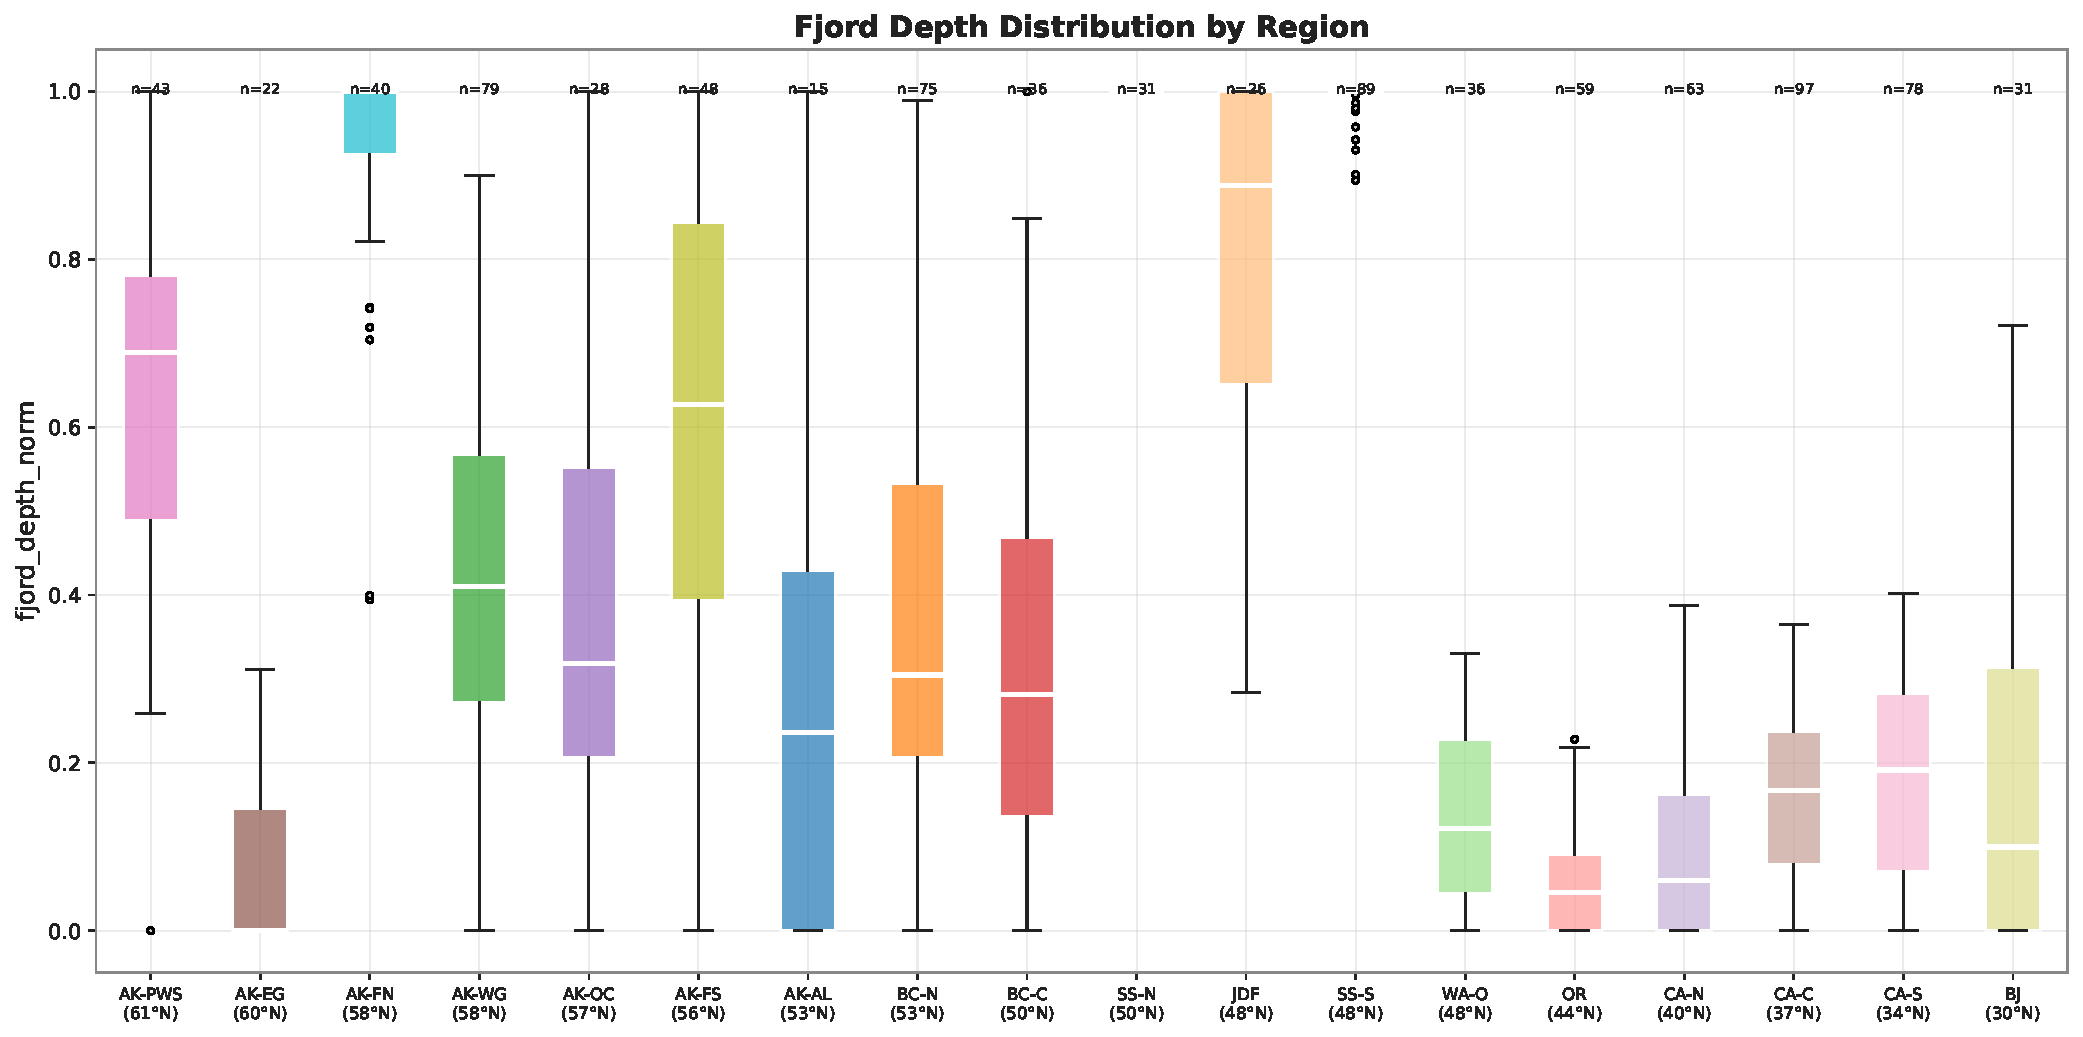
\includegraphics[width=0.85\textwidth]{fig_fjord_depth.pdf}
\caption{Distribution of \texttt{fjord\_depth\_norm} by region, ordered north to south. Alaskan fjord regions (AK-FN, AK-PWS, AK-FS) show high enclosedness, while California, Oregon, and Washington outer coast sites are uniformly low. Box plots show median, interquartile range, and outliers.}
\label{fig:fjord_depth}
\end{figure}

Notably, the Salish Sea regions (SS-N, SS-S) and Juan de Fuca (JDF) also show high \texttt{fjord\_depth\_norm} values (medians of 1.0, 1.0, and 0.888 respectively, with 100\%, 100\%, and 84.6\% above 0.5), indicating that these inland waterways are also predicted to experience substantial freshwater influence---consistent with the large Fraser River discharge.

% ============================================================
\section{Model Design}
\label{sec:model}
% ============================================================

\subsection{Core Equations}

The salinity model computes a time-varying salinity $S(\text{site}, \text{day})$ for each of the 896 nodes:

\begin{align}
\label{eq:salinity}
S(\text{site}, \text{day}) &= \max\!\big(s_{\text{floor}},\; S_{\text{ocean}}(\text{lat}) - \Delta S\big) \\
\label{eq:depression}
\Delta S &= \texttt{fw\_strength} \times \texttt{fd\_norm}^{\,\texttt{fw\_depth\_exp}} \times f_{\text{melt}}(\text{lat}) \times \texttt{melt\_pulse}(\text{day})
\end{align}

where:

\begin{itemize}[nosep]
    \item $S_{\text{ocean}}(\text{lat}) = 31.32 + 0.054 \times (\text{lat} - 50.0)$ --- latitudinally-varying ocean baseline salinity (psu)
    \item $\texttt{fw\_strength}$ --- maximum freshwater depression (psu); calibration parameter, range 6--25
    \item $\texttt{fd\_norm}$ --- site-specific fjord depth normalization ($0$--$1$); fixed per node
    \item $\texttt{fw\_depth\_exp}$ --- exponent controlling non-linearity of fjord depth effect; calibration parameter, range 0.3--3.0, default 1.0
    \item $f_{\text{melt}}(\text{lat})$ --- latitude-dependent melt factor
    \item $\texttt{melt\_pulse}(\text{day})$ --- seasonal melt timing function
    \item $s_{\text{floor}} = 5.0$ psu --- minimum salinity floor
\end{itemize}

\subsection{Component Functions}

The \textbf{latitude melt factor} scales the freshwater effect with latitude:
\begin{equation}
\label{eq:fmelt}
f_{\text{melt}}(\text{lat}) = \text{clip}\!\left(\frac{\text{lat} - 35}{25},\; 0,\; 1\right)
\end{equation}
This yields $f_{\text{melt}} = 0$ at latitudes $\leq 35$\textdegree N (southern California, Baja) and $f_{\text{melt}} = 1$ at latitudes $\geq 60$\textdegree N (Alaska), with linear interpolation between.

The \textbf{melt pulse} function creates a seasonal cycle peaking on day 166 (June 15):
\begin{equation}
\label{eq:melt_pulse}
\texttt{melt\_pulse}(\text{day}) = \max\!\left(0,\; \cos\!\left(\frac{2\pi(\text{day} - 166)}{365}\right)\right)
\end{equation}
This produces a half-cosine pulse that is positive from approximately mid-March to mid-September, with peak freshwater influence at the summer solstice.

Figure~\ref{fig:mechanism} illustrates these three components and their combined effect on salinity profiles at representative sites.

\begin{figure}[H]
\centering
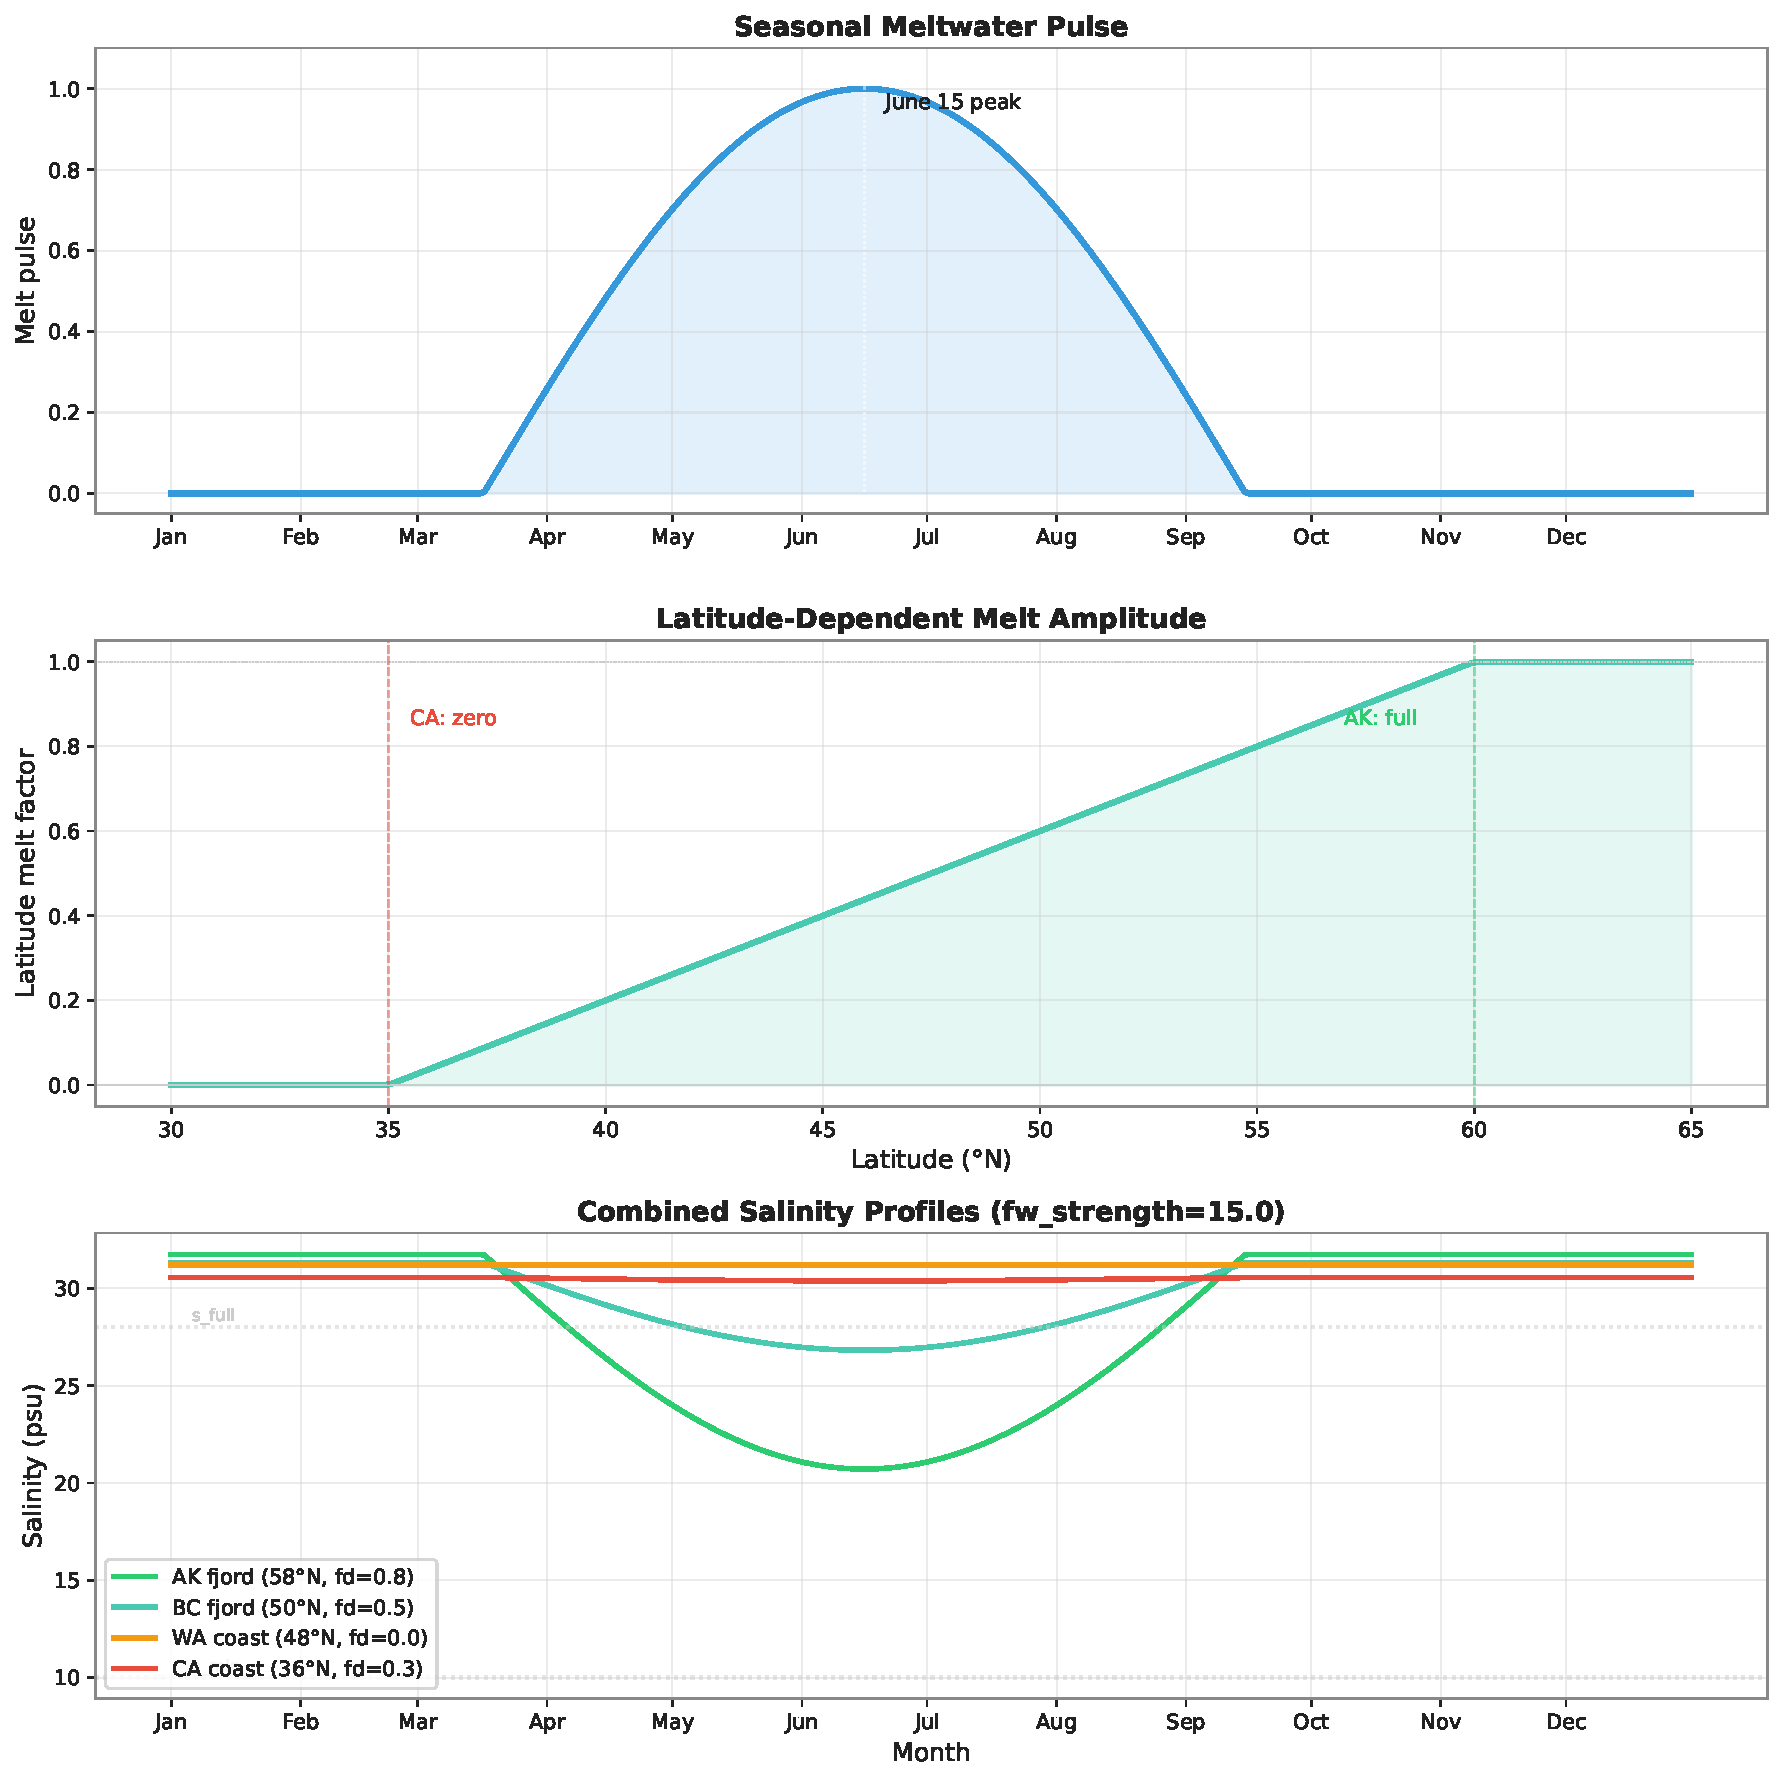
\includegraphics[width=0.95\textwidth]{fig_mechanism.pdf}
\caption{Three-panel mechanism overview. Left: seasonal melt pulse peaking on day 166. Center: latitude-dependent melt factor ($f_{\text{melt}}$) showing linear ramp from 35\textdegree N to 60\textdegree N. Right: combined seasonal salinity profiles for representative sites showing the interaction of all components.}
\label{fig:mechanism}
\end{figure}

\subsection{Salinity Modifier (Vibrio Response)}

The salinity effect on \textit{Vibrio} growth is modeled via a transfer function:
\begin{equation}
\label{eq:sal_mod}
\texttt{sal\_mod}(S) = \text{clip}\!\left(\left(\frac{S - s_{\text{min}}}{s_{\text{full}} - s_{\text{min}}}\right)^{\eta},\; 0,\; 1\right)
\end{equation}
with $s_{\text{min}} = 10.0$ psu (below which \textit{Vibrio} growth ceases), $s_{\text{full}} = 28.0$ psu (above which salinity is non-limiting), and $\eta = 2.0$ (curvature parameter giving a concave-up response). This means that moderate salinity reductions (e.g., from 32 to 25 psu) have relatively small effects, while drops below $\sim$20 psu cause rapid suppression.

\begin{figure}[H]
\centering
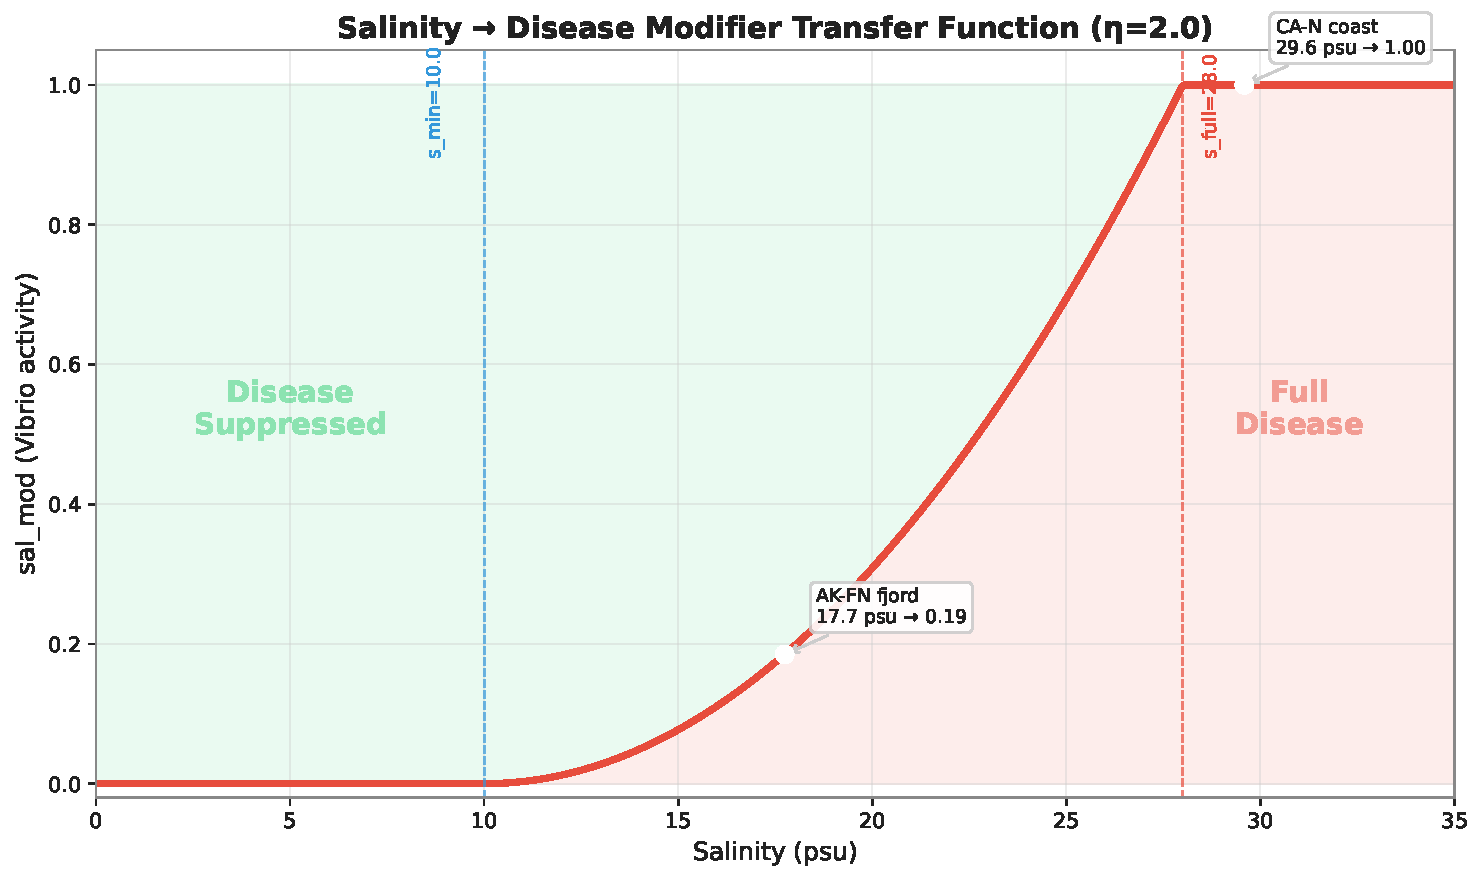
\includegraphics[width=0.75\textwidth]{fig_sal_mod.pdf}
\caption{Salinity modifier transfer function ($\texttt{sal\_mod}$) mapping salinity to \textit{Vibrio} growth capacity. Key thresholds: $s_{\text{min}} = 10$ psu (complete suppression), $s_{\text{full}} = 28$ psu (no limitation). The non-linear ($\eta = 2$) response means most suppression occurs below $\sim$22 psu. Annotated points show representative site salinities.}
\label{fig:sal_mod}
\end{figure}

\subsection{Backward Compatibility}

The model is fully backward-compatible with prior calibrations. Setting $\texttt{fw\_strength} = 0$ yields $\Delta S = 0$ for all sites and times, recovering the original constant-salinity model where $S(\text{site}) = S_{\text{ocean}}(\text{lat})$ year-round. The default value of \texttt{fw\_strength} is 0 (disabled), and the default \texttt{fw\_depth\_exp} is 1.0.

% ============================================================
\section{Spatial Predictions}
\label{sec:spatial}
% ============================================================

\subsection{The Alaska--California Asymmetry}

The central prediction of the salinity model is a dramatic asymmetry in disease suppression between Alaska and California. At \texttt{fw\_strength}~=~15, the mean June Vibrio suppression across 275 Alaskan nodes is 35.01\%, while across 238 California nodes it is exactly 0.0\%. This infinite asymmetry ratio arises because California sites combine low \texttt{fjord\_depth\_norm} (median 0.143 vs.\ Alaska's 0.493) with low latitude melt factors.

\begin{figure}[H]
\centering
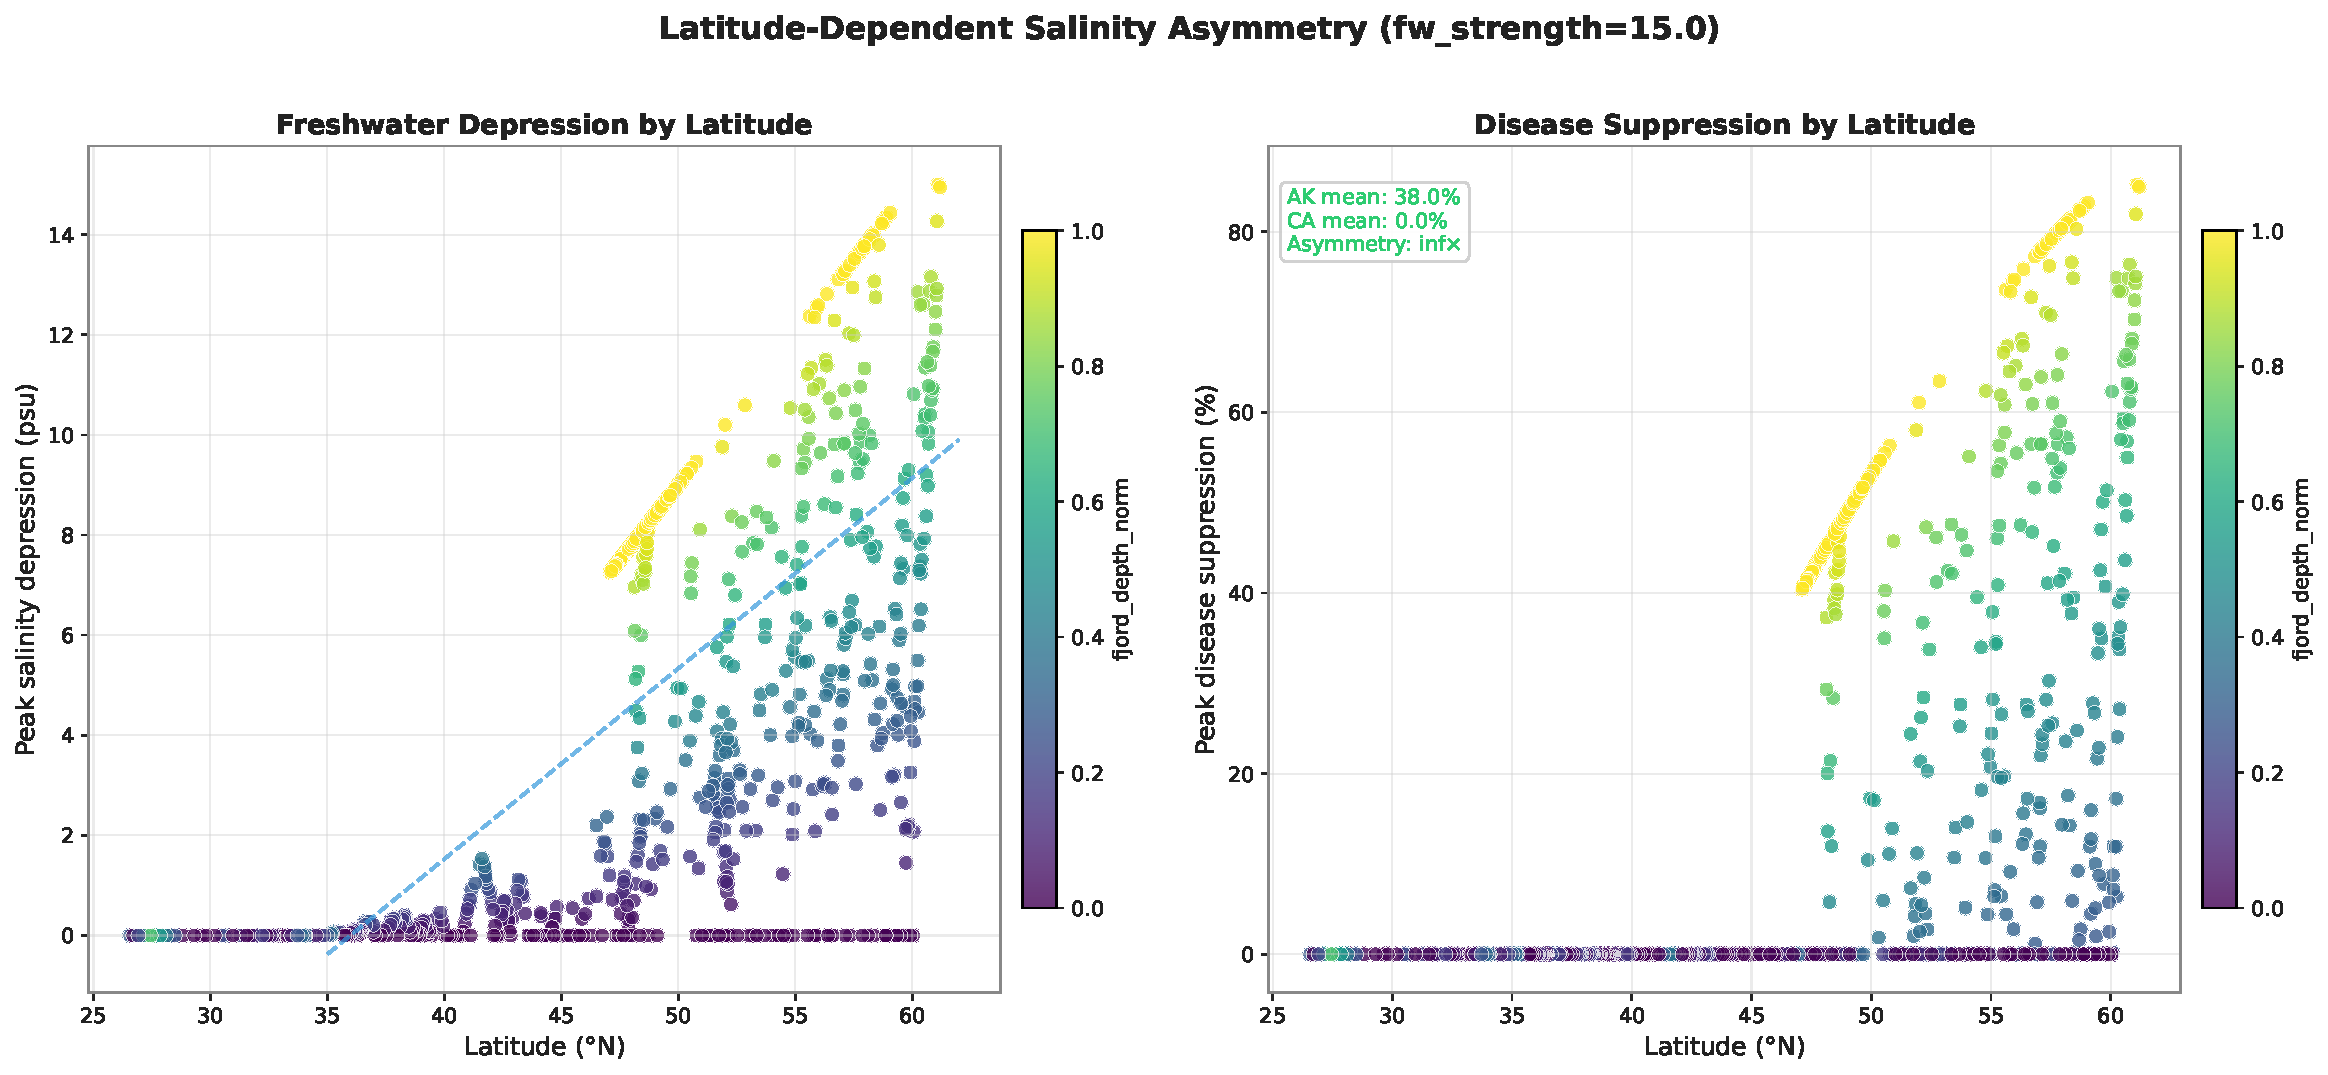
\includegraphics[width=0.95\textwidth]{fig_asymmetry.pdf}
\caption{Two-panel latitude asymmetry diagnostic at \texttt{fw\_strength}~=~15. Left: mean June salinity depression (psu) by latitude, showing the strong high-latitude signal driven by fjord depth and melt factor. Right: mean June Vibrio suppression (\%) by latitude, demonstrating the non-linear amplification through the $\texttt{sal\_mod}$ transfer function.}
\label{fig:asymmetry}
\end{figure}

\subsection{Regional Patterns}

Table~\ref{tab:regional} summarizes predictions across all 18 regions at \texttt{fw\_strength}~=~15.

\begin{table}[H]
\centering
\small
\caption{Regional summary of salinity mechanism predictions at \texttt{fw\_strength}~=~15. Depression and suppression refer to June peak values.}
\label{tab:regional}
\begin{tabular}{lrcccccc}
\toprule
Region & $n$ & Lat & $\overline{\texttt{fd}}$ & June $S$ (psu) & $\Delta S$ (psu) & Suppr.\ (\%) & Max Suppr.\ (\%) \\
\midrule
AK-PWS & 43  & 60.6 & 0.633 & 22.4  & 9.49  & 50.3  & 85.2 \\
AK-EG  & 22  & 59.6 & 0.087 & 30.5  & 1.30  & 0.8   & 8.8 \\
AK-FN  & 40  & 57.9 & 0.927 & 19.0  & 12.76 & 73.7  & 83.2 \\
AK-WG  & 79  & 57.8 & 0.402 & 26.2  & 5.56  & 23.7  & 74.9 \\
AK-OC  & 28  & 57.1 & 0.378 & 26.6  & 5.10  & 21.0  & 82.8 \\
AK-FS  & 48  & 55.8 & 0.617 & 23.9  & 7.73  & 38.7  & 77.3 \\
AK-AL  & 15  & 52.9 & 0.287 & 28.5  & 3.02  & 11.9  & 61.1 \\
BC-N   & 75  & 52.5 & 0.365 & 27.6  & 3.89  & 12.2  & 63.5 \\
BC-C   & 36  & 50.2 & 0.315 & 28.4  & 2.91  & 8.1   & 54.7 \\
SS-N   & 31  & 49.6 & 1.000 & 22.5  & 8.78  & 51.6  & 56.3 \\
JDF    & 26  & 48.0 & 0.804 & 25.0  & 6.25  & 30.5  & 45.5 \\
SS-S   & 89  & 48.0 & 0.995 & 23.4  & 7.77  & 44.2  & 48.9 \\
WA-O   & 36  & 47.6 & 0.133 & 30.2  & 1.00  & 0.0   & 0.0 \\
OR     & 59  & 43.9 & 0.056 & 30.7  & 0.28  & 0.0   & 0.0 \\
CA-N   & 63  & 40.1 & 0.101 & 30.4  & 0.36  & 0.0   & 0.0 \\
CA-C   & 97  & 36.7 & 0.155 & 30.5  & 0.15  & 0.0   & 0.0 \\
CA-S   & 78  & 33.6 & 0.182 & 30.4  & 0.00  & 0.0   & 0.0 \\
BJ     & 31  & 29.6 & 0.186 & 30.2  & 0.00  & 0.0   & 0.0 \\
\bottomrule
\end{tabular}
\end{table}

Several patterns merit attention:

\begin{itemize}
    \item \textbf{AK-FN dominates:} With the highest mean \texttt{fjord\_depth\_norm} (0.927) and 95\% of nodes above 0.5, AK-FN shows the largest mean depression (12.76 psu) and suppression (73.7\%).
    \item \textbf{AK-EG is an outlier:} Despite high latitude (59.6\textdegree N), AK-EG's low \texttt{fjord\_depth\_norm} (0.087, median 0.0, 0\% above 0.5) yields minimal suppression (0.8\%)---illustrating that latitude alone is insufficient.
    \item \textbf{Salish Sea is strongly affected:} SS-N and SS-S, despite lower latitudes ($\sim$48--50\textdegree N), show 51.6\% and 44.2\% mean suppression due to maximal \texttt{fjord\_depth\_norm} (1.0 and 0.995 respectively).
    \item \textbf{Sharp southern cutoff:} WA-O, OR, and all California regions show 0.0\% suppression, creating a sharp transition around 47--48\textdegree N.
\end{itemize}

\begin{figure}[H]
\centering
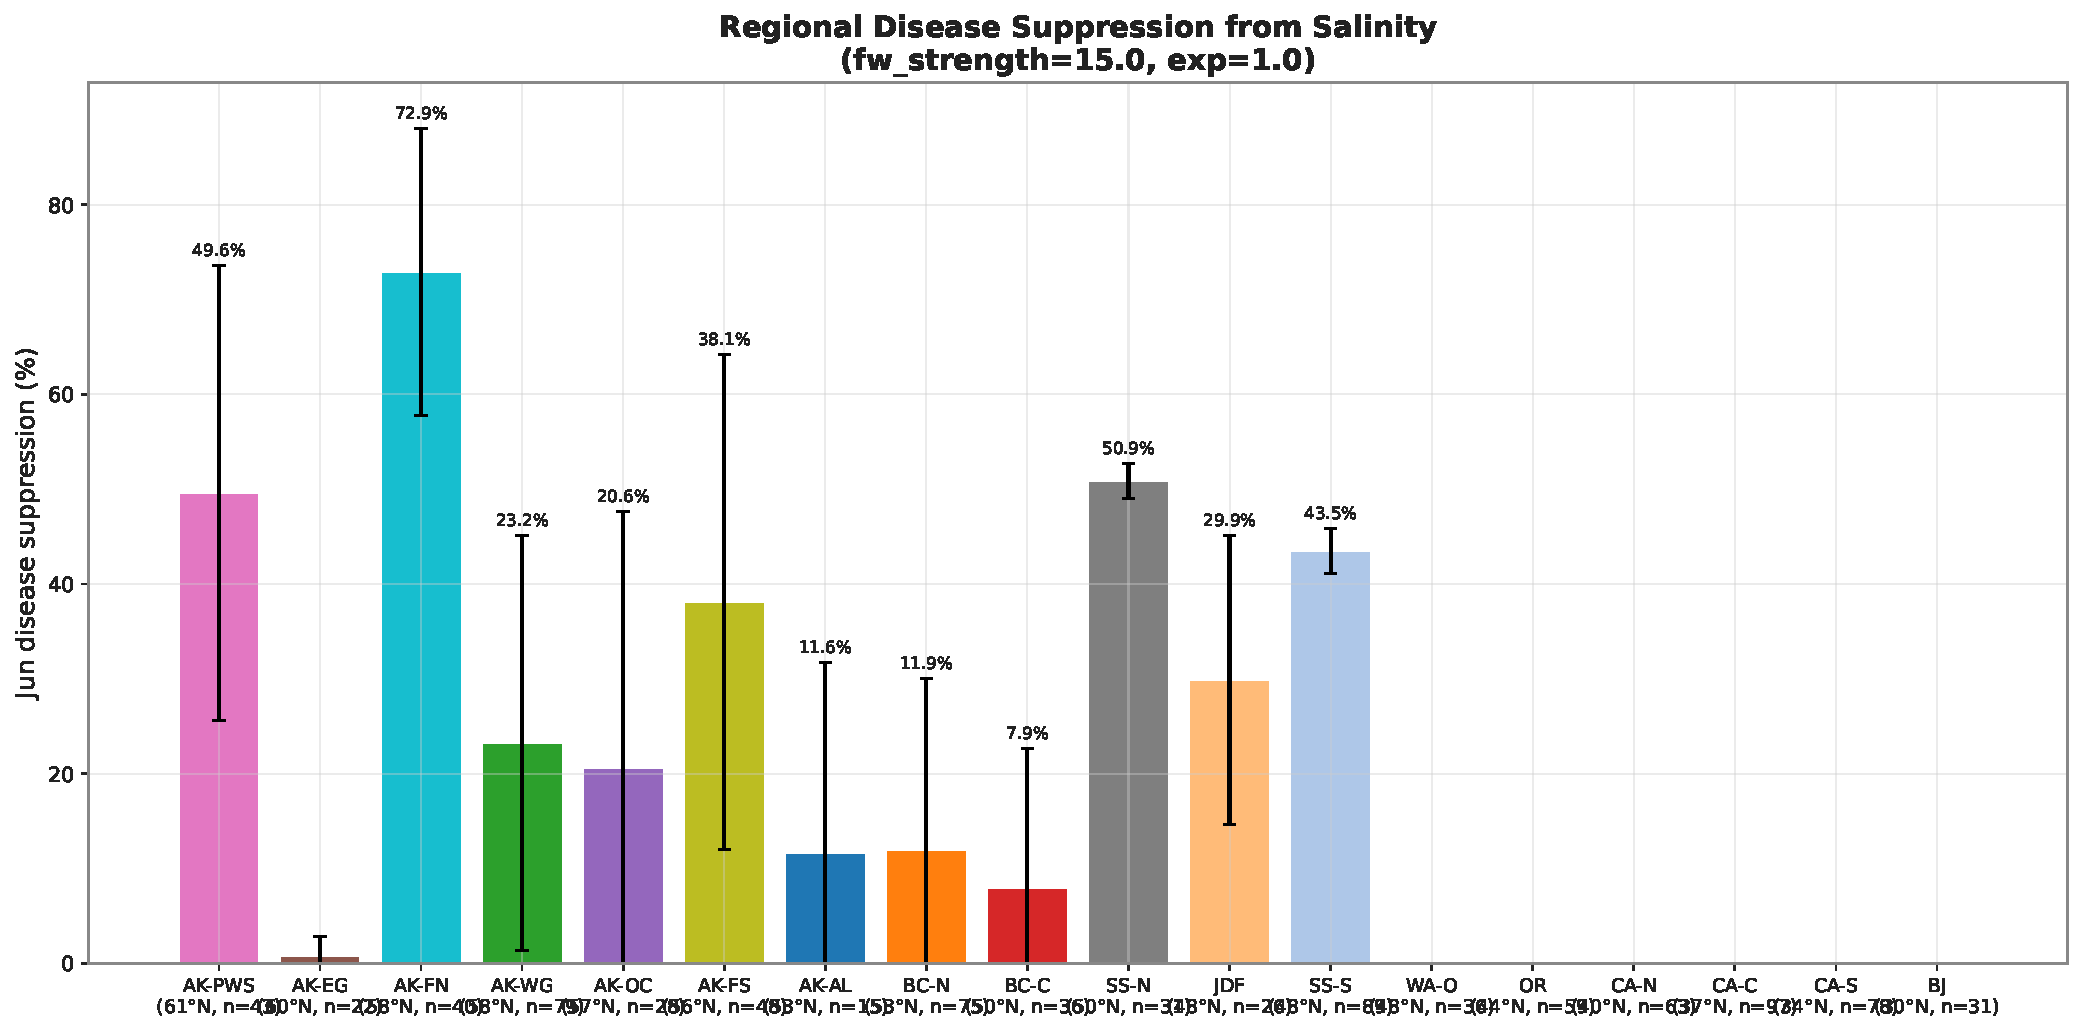
\includegraphics[width=0.85\textwidth]{fig_suppression_bars.pdf}
\caption{Mean June Vibrio suppression (\%) by region at \texttt{fw\_strength}~=~15, ordered north to south. The gradient from AK-FN (73.7\%) through BC to zero suppression south of the Salish Sea is clearly visible.}
\label{fig:suppression_bars}
\end{figure}

\subsection{Seasonal Dynamics}

The melt pulse function (Eq.~\ref{eq:melt_pulse}) creates a distinct seasonal pattern in salinity depression. Figure~\ref{fig:regional_profiles} shows the full annual salinity cycle for each region, illustrating how the summer trough depth and duration vary with latitude and fjord depth.

\begin{figure}[H]
\centering

\includegraphics[width=0.95\textwidth]{fig_regional_profiles.pdf}
\caption{Seasonal salinity curves by region at \texttt{fw\_strength}~=~15. Each curve shows the mean salinity across all nodes in the region. The deepest summer troughs occur in AK-FN (reaching $\sim$19 psu) and SS-N ($\sim$22.5 psu). California and Oregon regions show near-constant salinity year-round.}
\label{fig:regional_profiles}
\end{figure}

The spatial evolution of suppression through the year is shown in Figure~\ref{fig:monthly_panels}, revealing how the suppression zone expands from initial appearance in April--May through peak coverage in June--July, then contracts by September.

\begin{figure}[H]
\centering
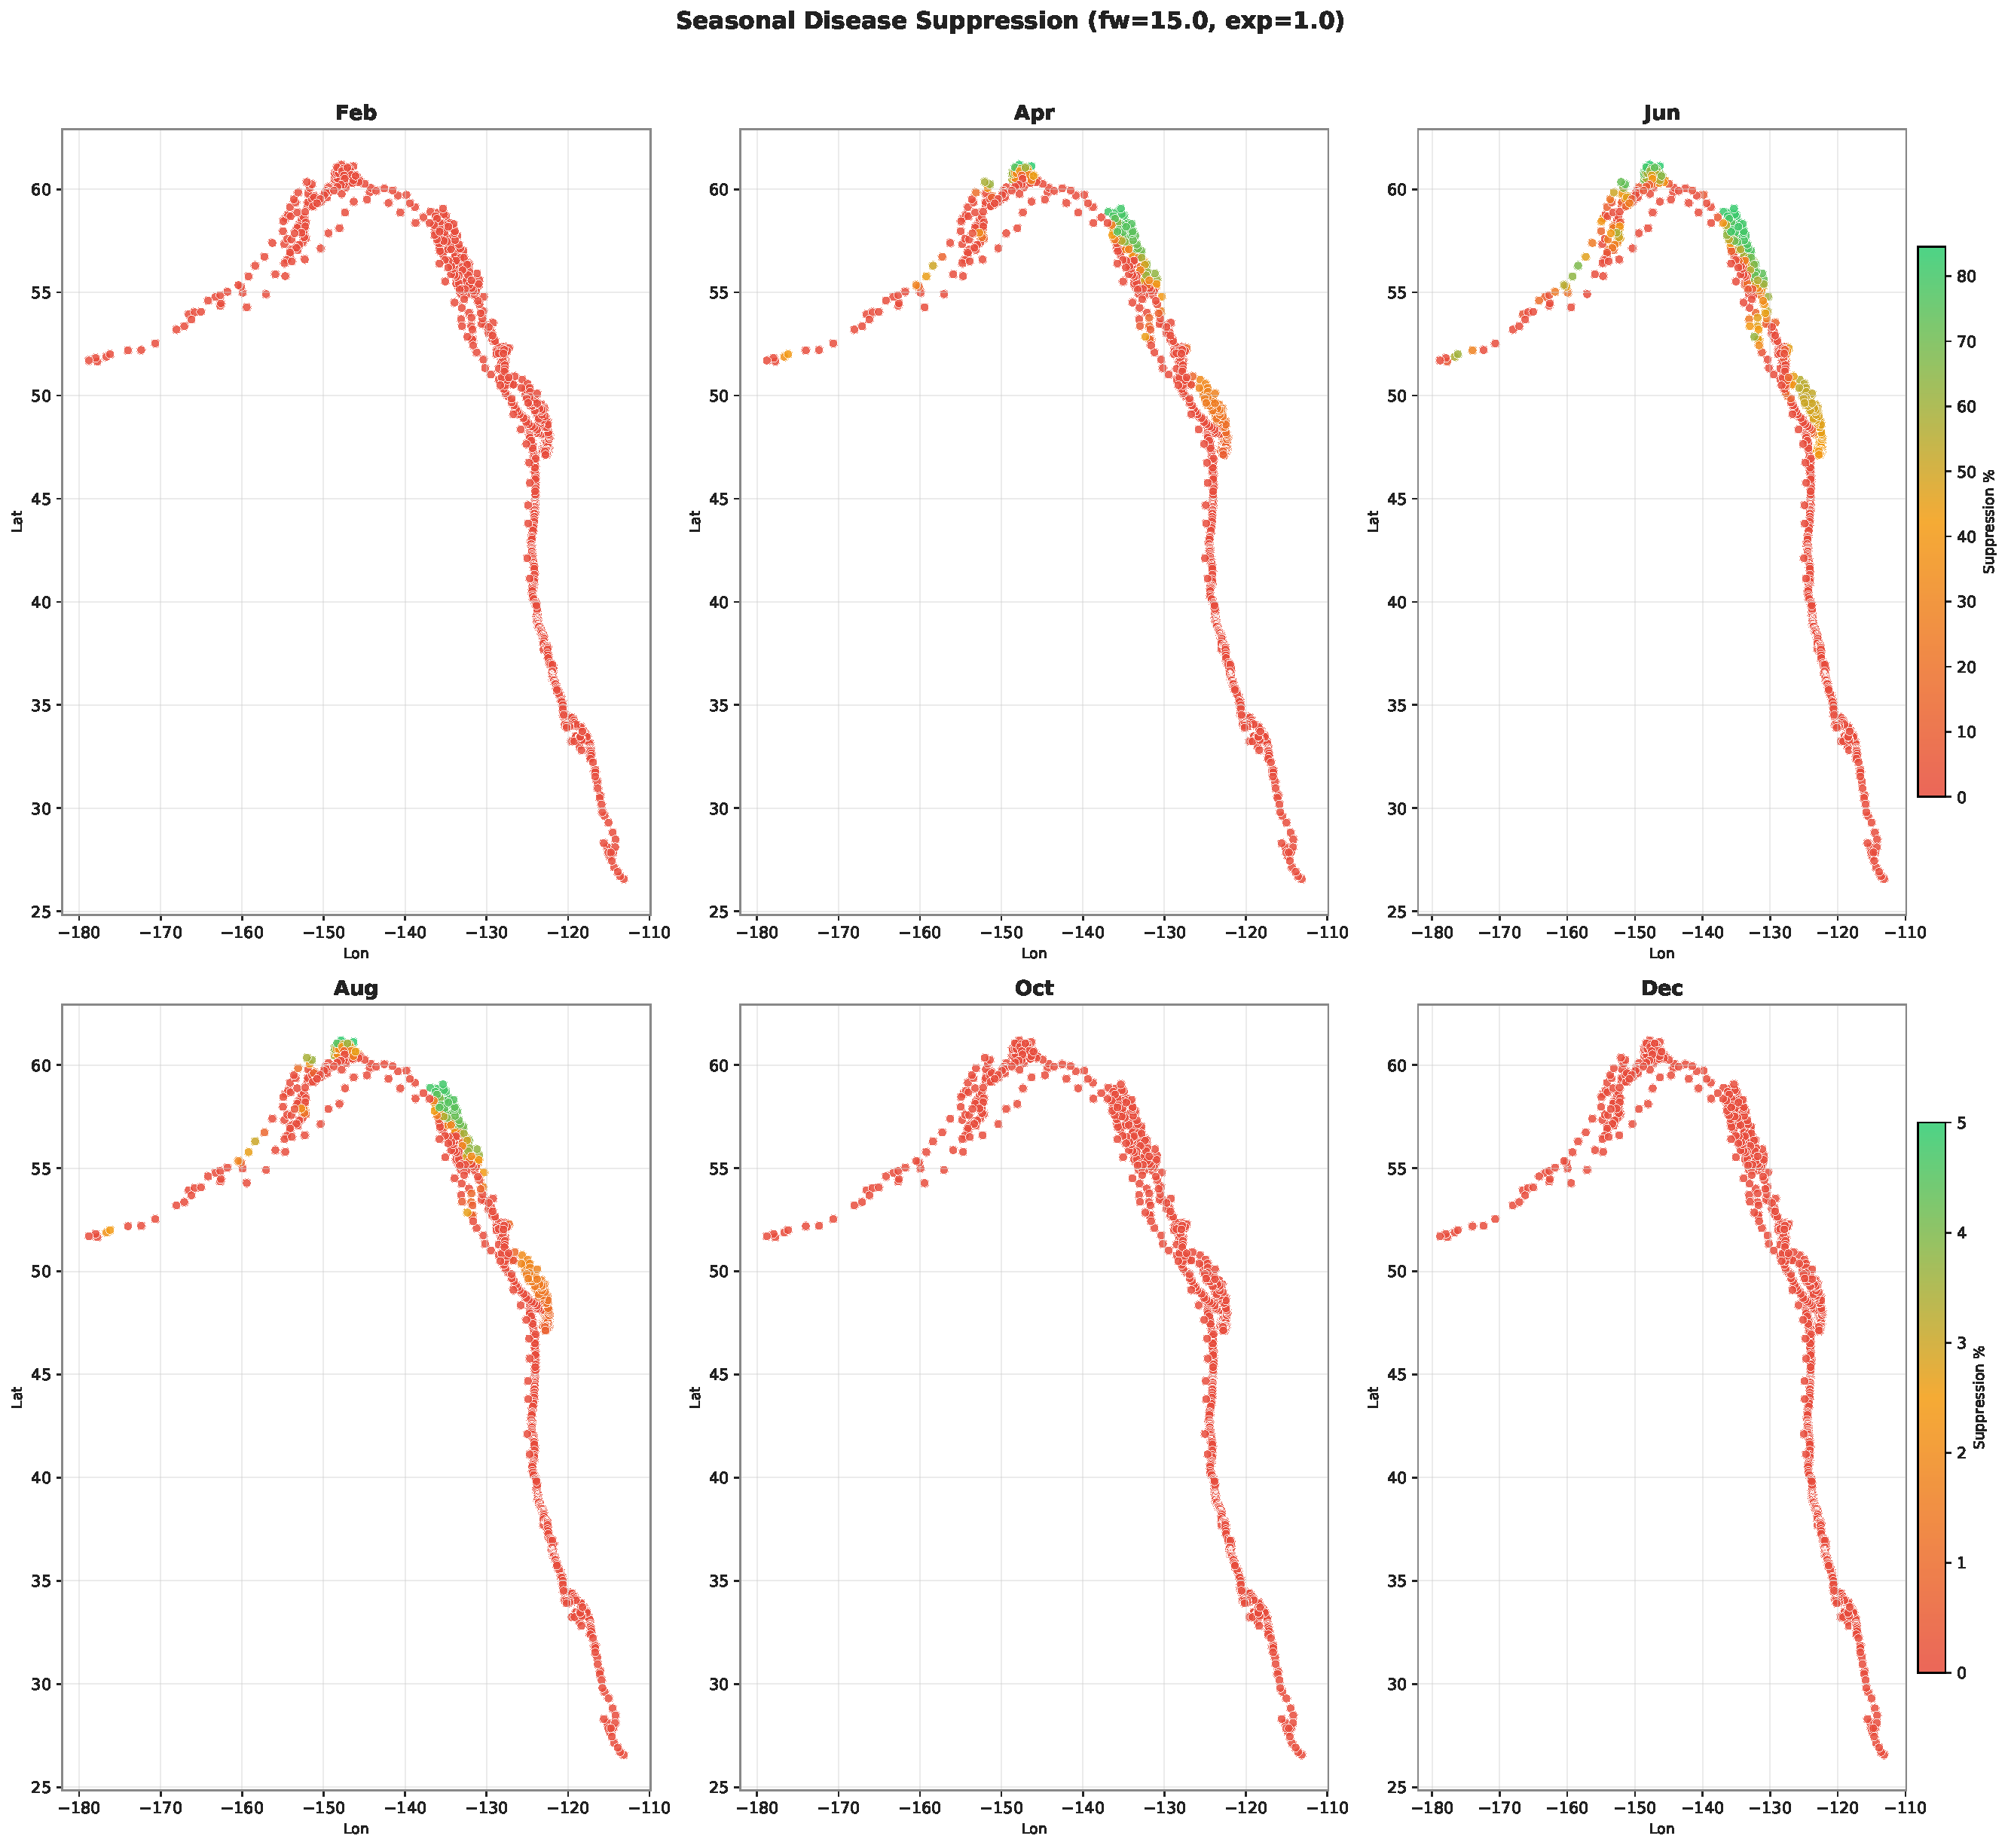
\includegraphics[width=0.95\textwidth]{fig_monthly_panels.pdf}
\caption{Geographic maps of Vibrio suppression by month (6 panels covering the melt season). Suppression is concentrated in Alaskan fjords and the Salish Sea, peaking in June--July and disappearing by October.}
\label{fig:monthly_panels}
\end{figure}

\subsection{Site-Level Depression Patterns}

Figure~\ref{fig:depression_heatmap} shows the top 50 sites by total salinity depression, revealing the monthly timing and intensity of the freshwater effect at the node level.

\begin{figure}[H]
\centering
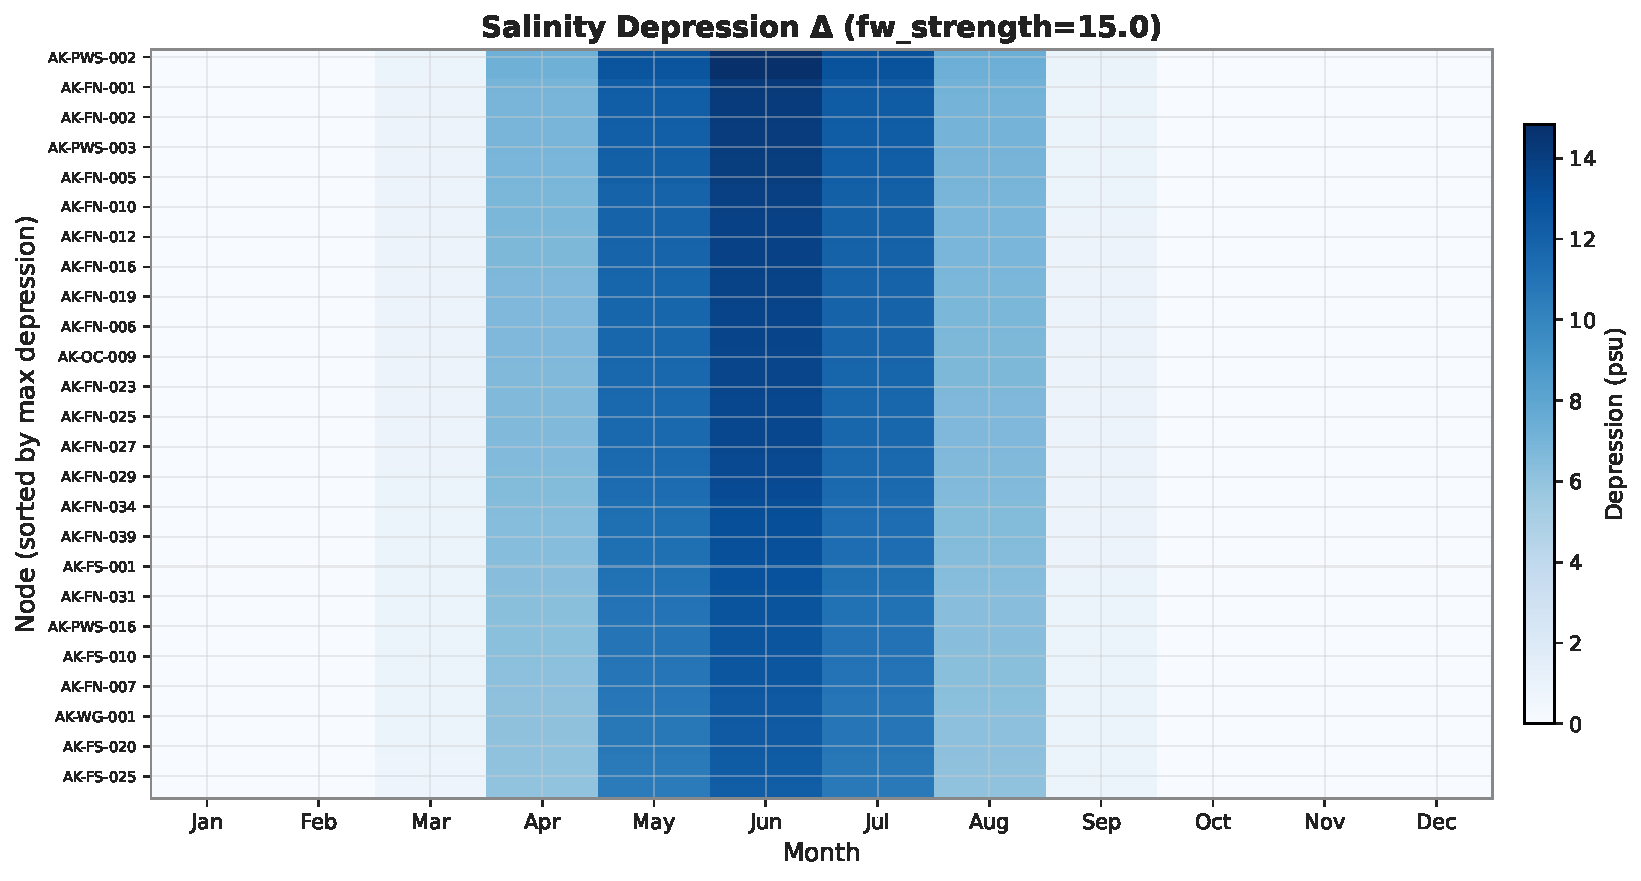
\includegraphics[width=0.95\textwidth]{fig_depression_heatmap.pdf}
\caption{Heatmap of salinity depression ($\Delta S$, psu) for the top 50 most-affected sites across months. Peak depression at AK-PWS-002 reaches 15.0 psu in June. The symmetric melt pulse shape is visible in the temporal pattern.}
\label{fig:depression_heatmap}
\end{figure}

The most extreme case is node AK-PWS-002 at 61.11\textdegree N with $\texttt{fd\_norm} = 1.0$, which experiences a peak June depression of 15.0 psu, driving salinity from the ocean baseline of $\sim$31.9 psu down to $\sim$16.9 psu.

To illustrate the Alaska--California contrast at the individual site level, consider two representative nodes:
\begin{itemize}[nosep]
    \item \textbf{AK-FN-008} (58.38\textdegree N, $\texttt{fd\_norm} = 1.0$): June salinity drops to 17.74~psu at \texttt{fw\_strength}~=~15, deep in the suppression zone of the $\texttt{sal\_mod}$ curve.
    \item \textbf{CA-N-006} (41.75\textdegree N, $\texttt{fd\_norm} = 0.319$): June salinity remains at 29.58~psu---above $s_{\text{full}}$, entirely unaffected.
\end{itemize}

\subsection{Regional Detail: Zoomed Views}
\label{sec:regional_zoom}

The preceding network-wide summaries reveal the broad latitude gradient, but mask important intra-regional heterogeneity. To resolve individual-site behavior, we present three complementary zoomed diagnostics covering four focal regions: Alaska (AK-FN, AK-PWS, AK-FS), British Columbia (BC-N, BC-C), Salish Sea / Juan de Fuca (SS-N, SS-S, JDF), and Oregon / California (OR, CA-N, CA-C).

\paragraph{Suppression by site within regions.}
Figure~\ref{fig:regional_zoom} decomposes the regional bar-chart summary (Figure~\ref{fig:suppression_bars}) into individual sites. Within Alaska, AK-FN shows a tight cluster of sites near 70--80\% suppression, reflecting its uniformly high \texttt{fjord\_depth\_norm}. AK-PWS is more heterogeneous, ranging from 0\% (exposed outer-coast nodes) to $>$85\% (inner Prince William Sound fjords). The Salish Sea panels reveal that SS-N and SS-S nodes are tightly clustered around 45--55\% suppression, consistent with their near-uniform $\texttt{fd\_norm} \approx 1.0$. Oregon and California panels confirm complete absence of suppression across all nodes.

\begin{figure}[H]
\centering

\includegraphics[width=0.95\textwidth]{fig_regional_zoom.pdf}
\caption{Regional zoom: June Vibrio suppression (\%) at individual sites within four focal region groups. Each dot represents a single model node; horizontal spread is for visibility. Alaska shows large intra-regional spread driven by fjord depth variation, while Salish Sea and southern regions are more homogeneous.}
\label{fig:regional_zoom}
\end{figure}

\paragraph{Regional salinity profiles at site resolution.}
Figure~\ref{fig:regional_sal_profiles} shows the full annual salinity cycle for every node in each focal region, overlaid as semi-transparent traces. This reveals the \emph{envelope} of salinity variability: in AK-FN, individual traces range from 17~psu to 24~psu at the June minimum, while in BC the envelope is narrower (27--30~psu). The Salish Sea panels show remarkably uniform seasonal cycles across sites, consistent with strong tidal mixing in a shared water body. Southern regions display flat, overlapping traces near 30.5~psu year-round.

\begin{figure}[H]
\centering
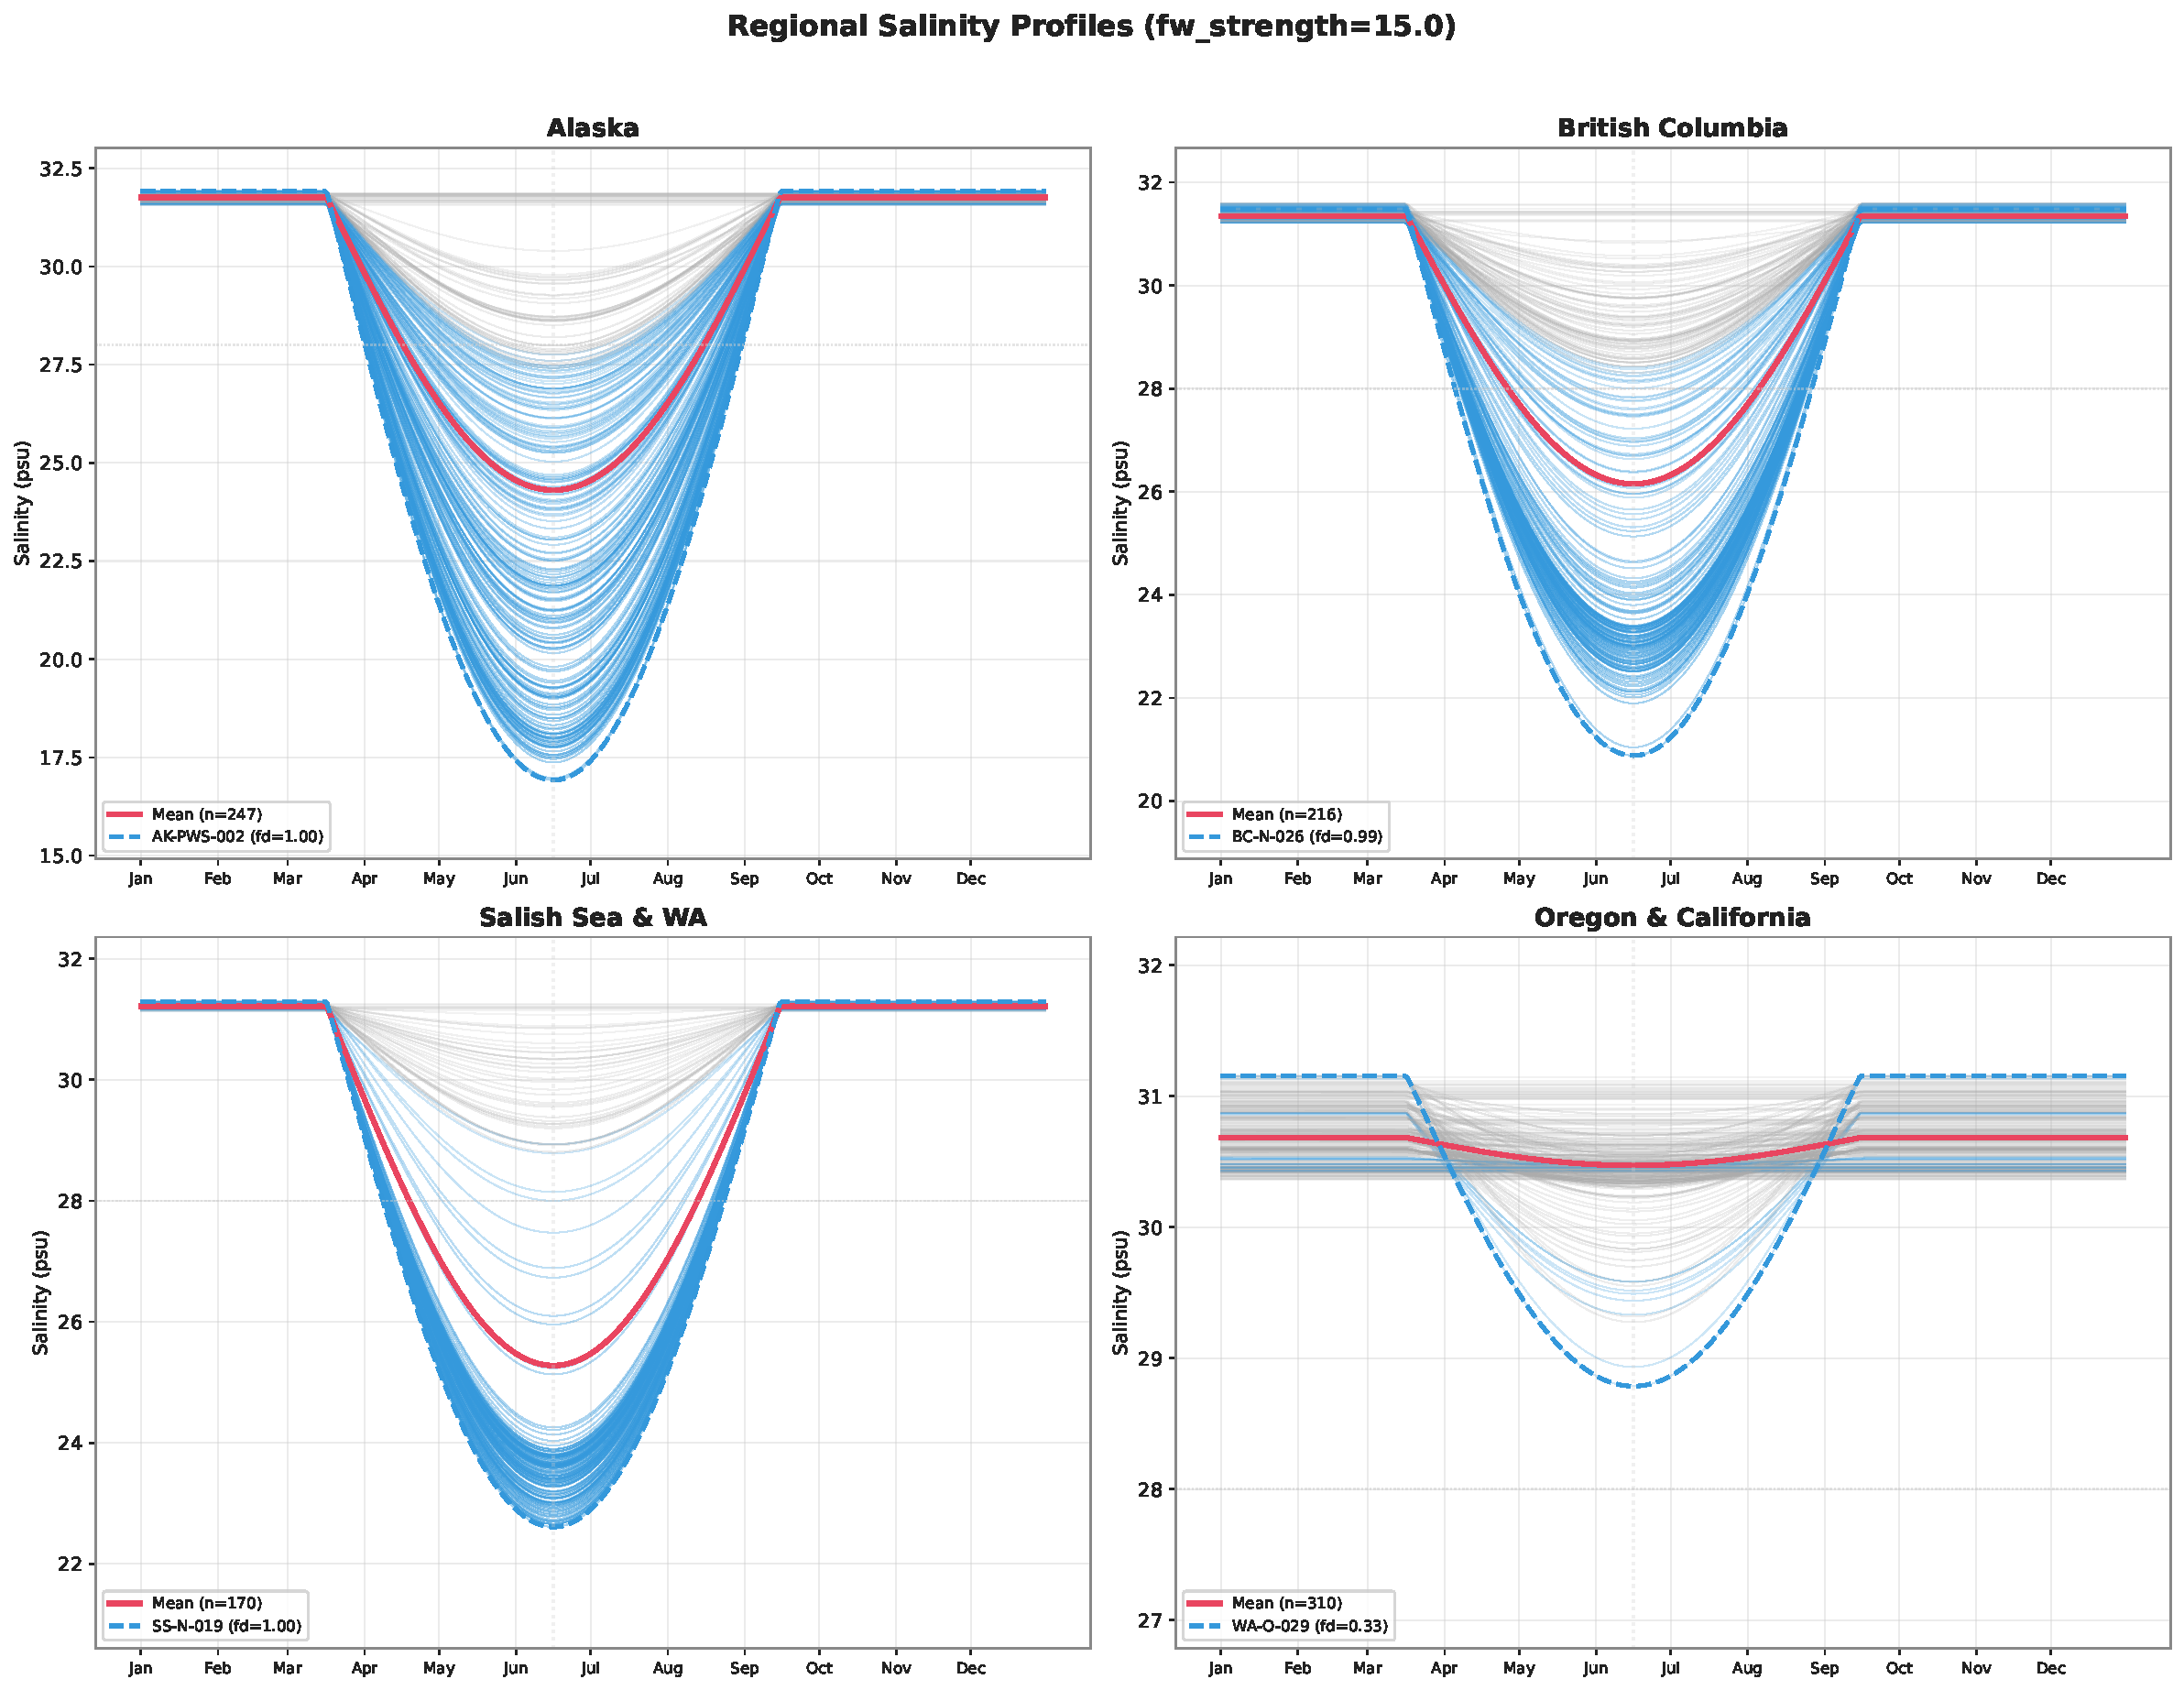
\includegraphics[width=0.95\textwidth]{fig_regional_sal_profiles.pdf}
\caption{Regional zoom: annual salinity profiles for every node in each focal region. Thin traces show individual sites; thick line shows regional mean. The spread of traces quantifies intra-regional heterogeneity in freshwater exposure.}
\label{fig:regional_sal_profiles}
\end{figure}

\paragraph{Depression--depth scatter.}
Figure~\ref{fig:depression_scatter} plots peak June salinity depression against \texttt{fjord\_depth\_norm} for each node, colored by region group. The power-law relationship $\Delta S \propto \texttt{fd\_norm}^{\texttt{fw\_depth\_exp}}$ is clearly visible, with the latitude melt factor $f_{\text{melt}}$ separating the Alaska and BC/Salish Sea point clouds vertically. The scatter confirms that fjord depth is the dominant within-region predictor of freshwater exposure, while latitude scales the overall magnitude.

\begin{figure}[H]
\centering
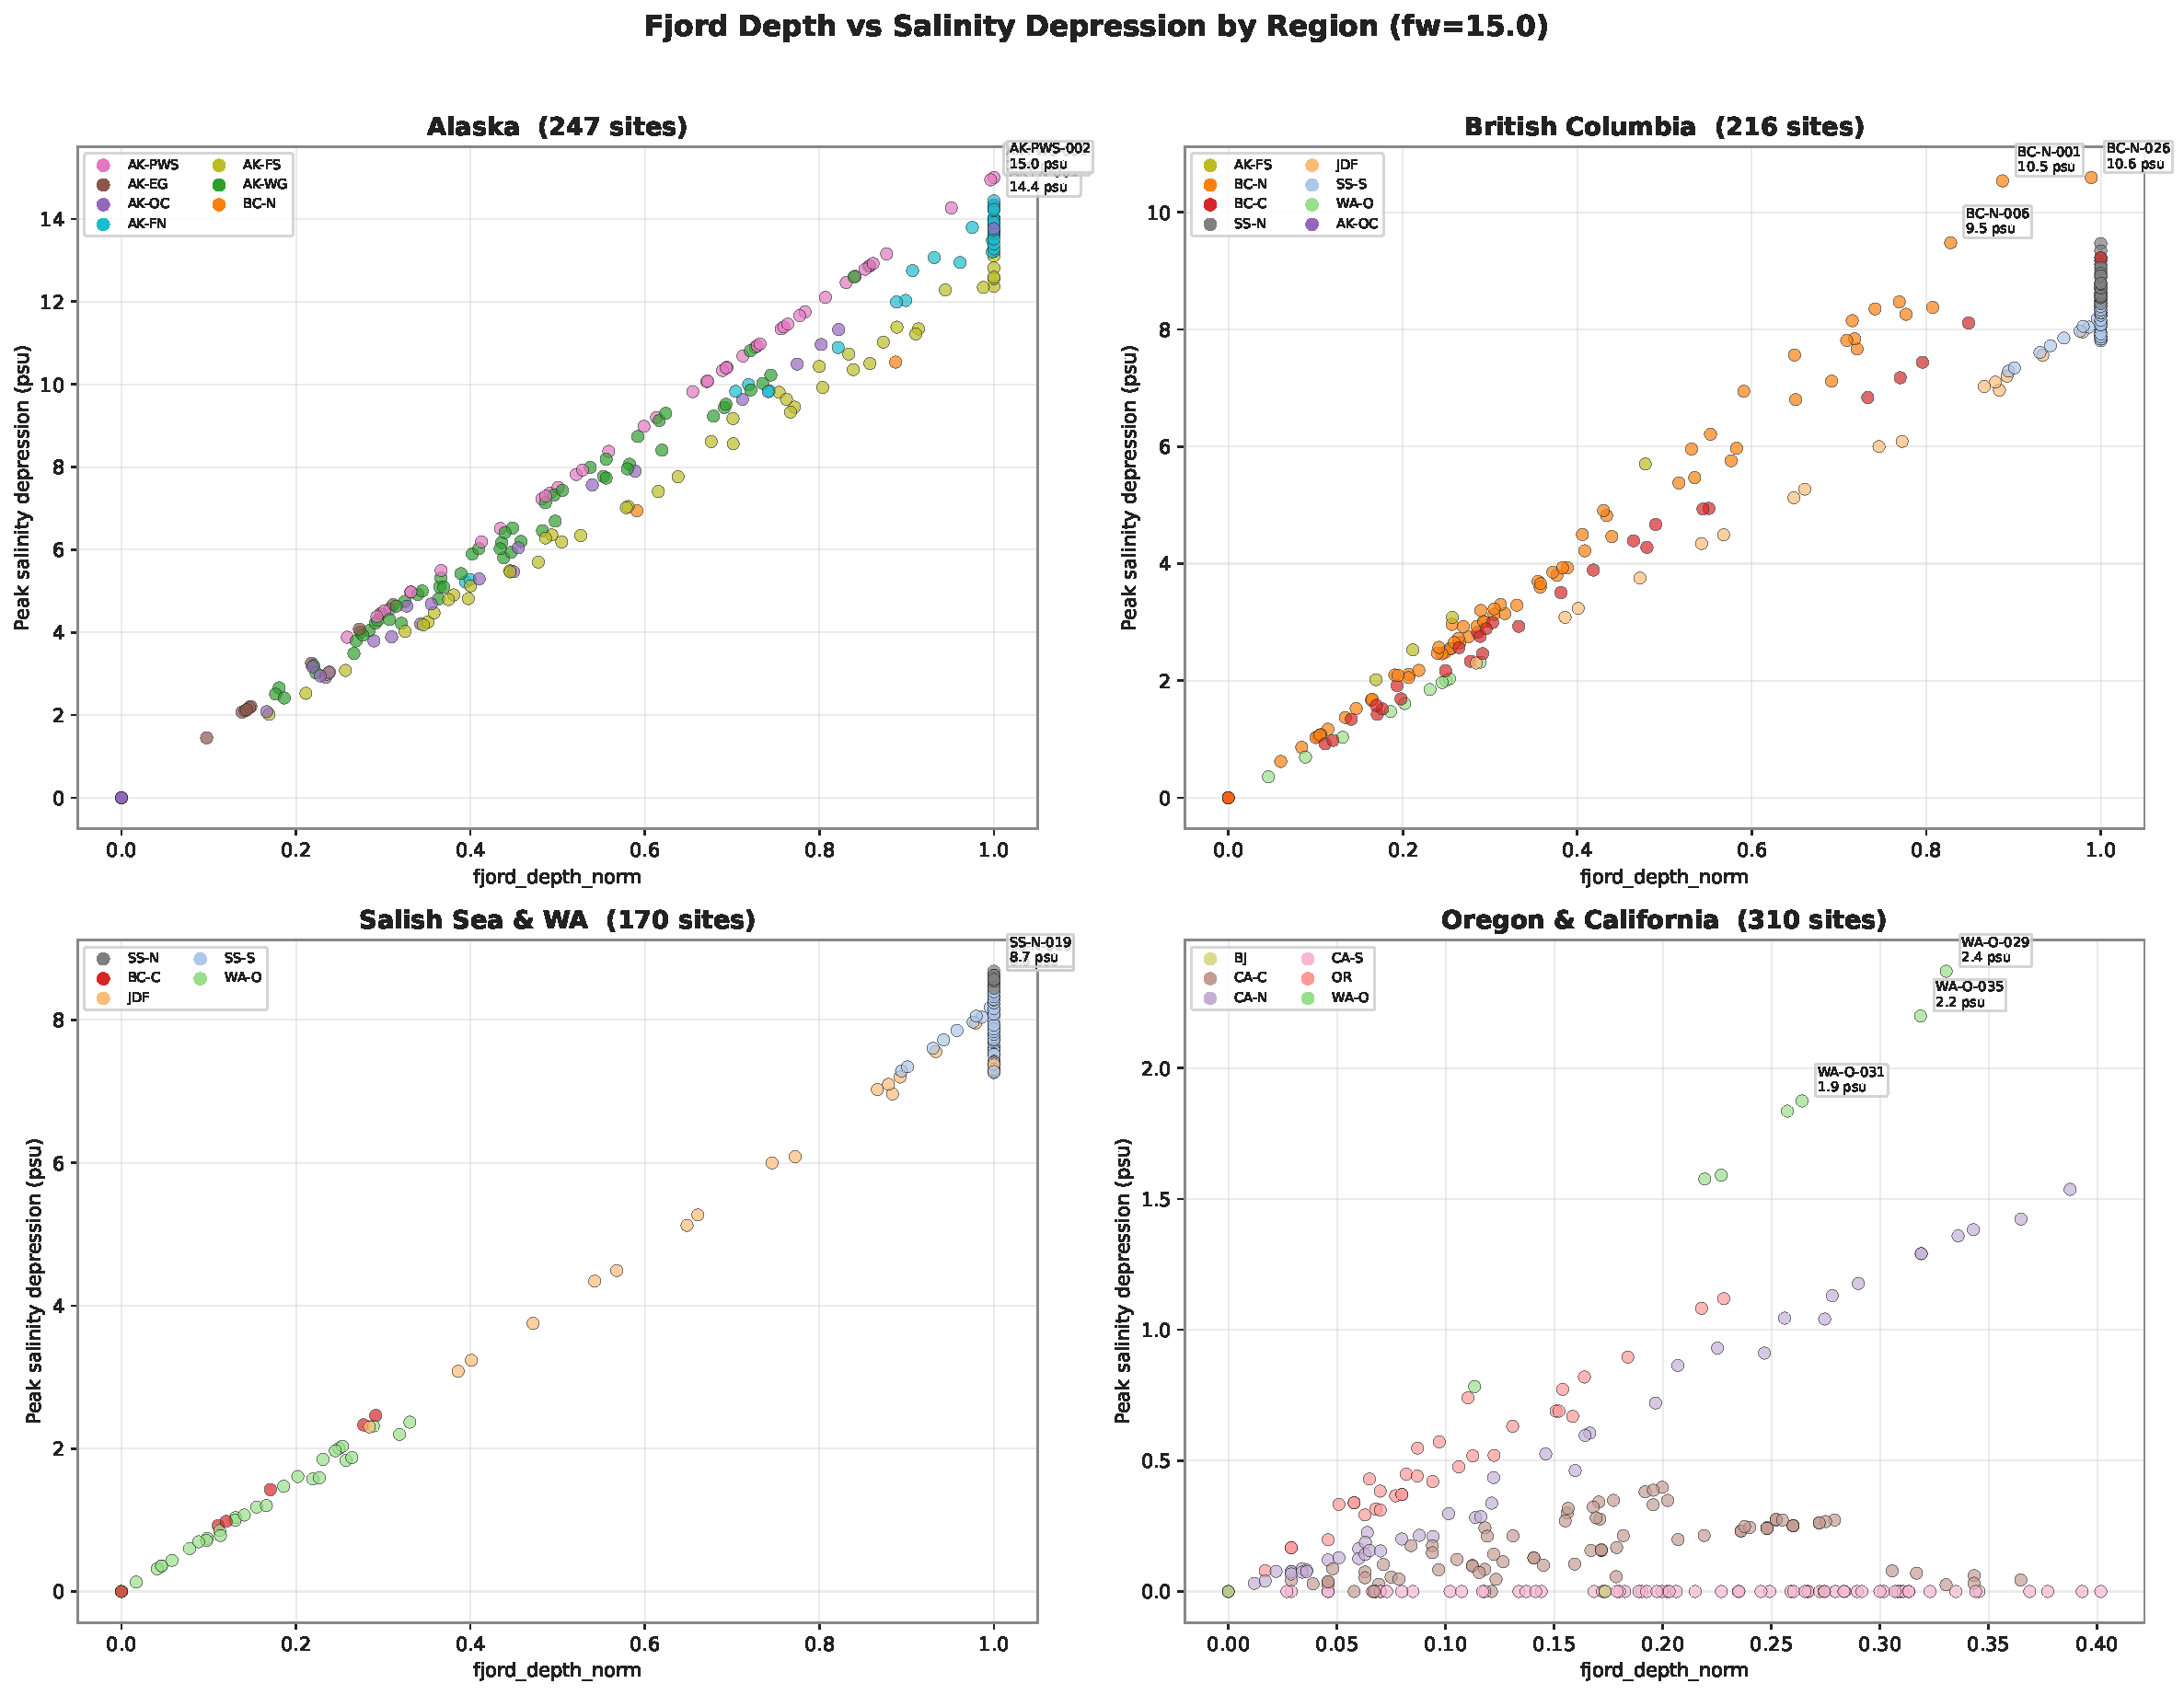
\includegraphics[width=0.85\textwidth]{fig_depression_scatter.pdf}
\caption{Regional zoom: peak June salinity depression (psu) vs.\ \texttt{fjord\_depth\_norm} for all nodes, colored by region group. The power-law envelope reflects the $\texttt{fd\_norm}^{\texttt{fw\_depth\_exp}}$ term; vertical separation between Alaskan and southern point clouds reflects the latitude melt factor.}
\label{fig:depression_scatter}
\end{figure}

These zoomed views highlight that the salinity mechanism creates \emph{structured heterogeneity} within regions, not merely a north--south gradient. This within-region variation is potentially diagnostic during calibration: sites in the same region but at different fjord depths should show differential disease dynamics if the salinity mechanism is operative.

% ============================================================
\section{Sensitivity Analysis}
\label{sec:sensitivity}
% ============================================================

\subsection{fw\_strength Dose-Response}

The \texttt{fw\_strength} parameter controls the magnitude of freshwater depression and is expected to be the primary calibration lever. Its range (6--25 psu) was chosen to span from minimal detectable effect to extreme freshwater dominance.

\begin{figure}[H]
\centering
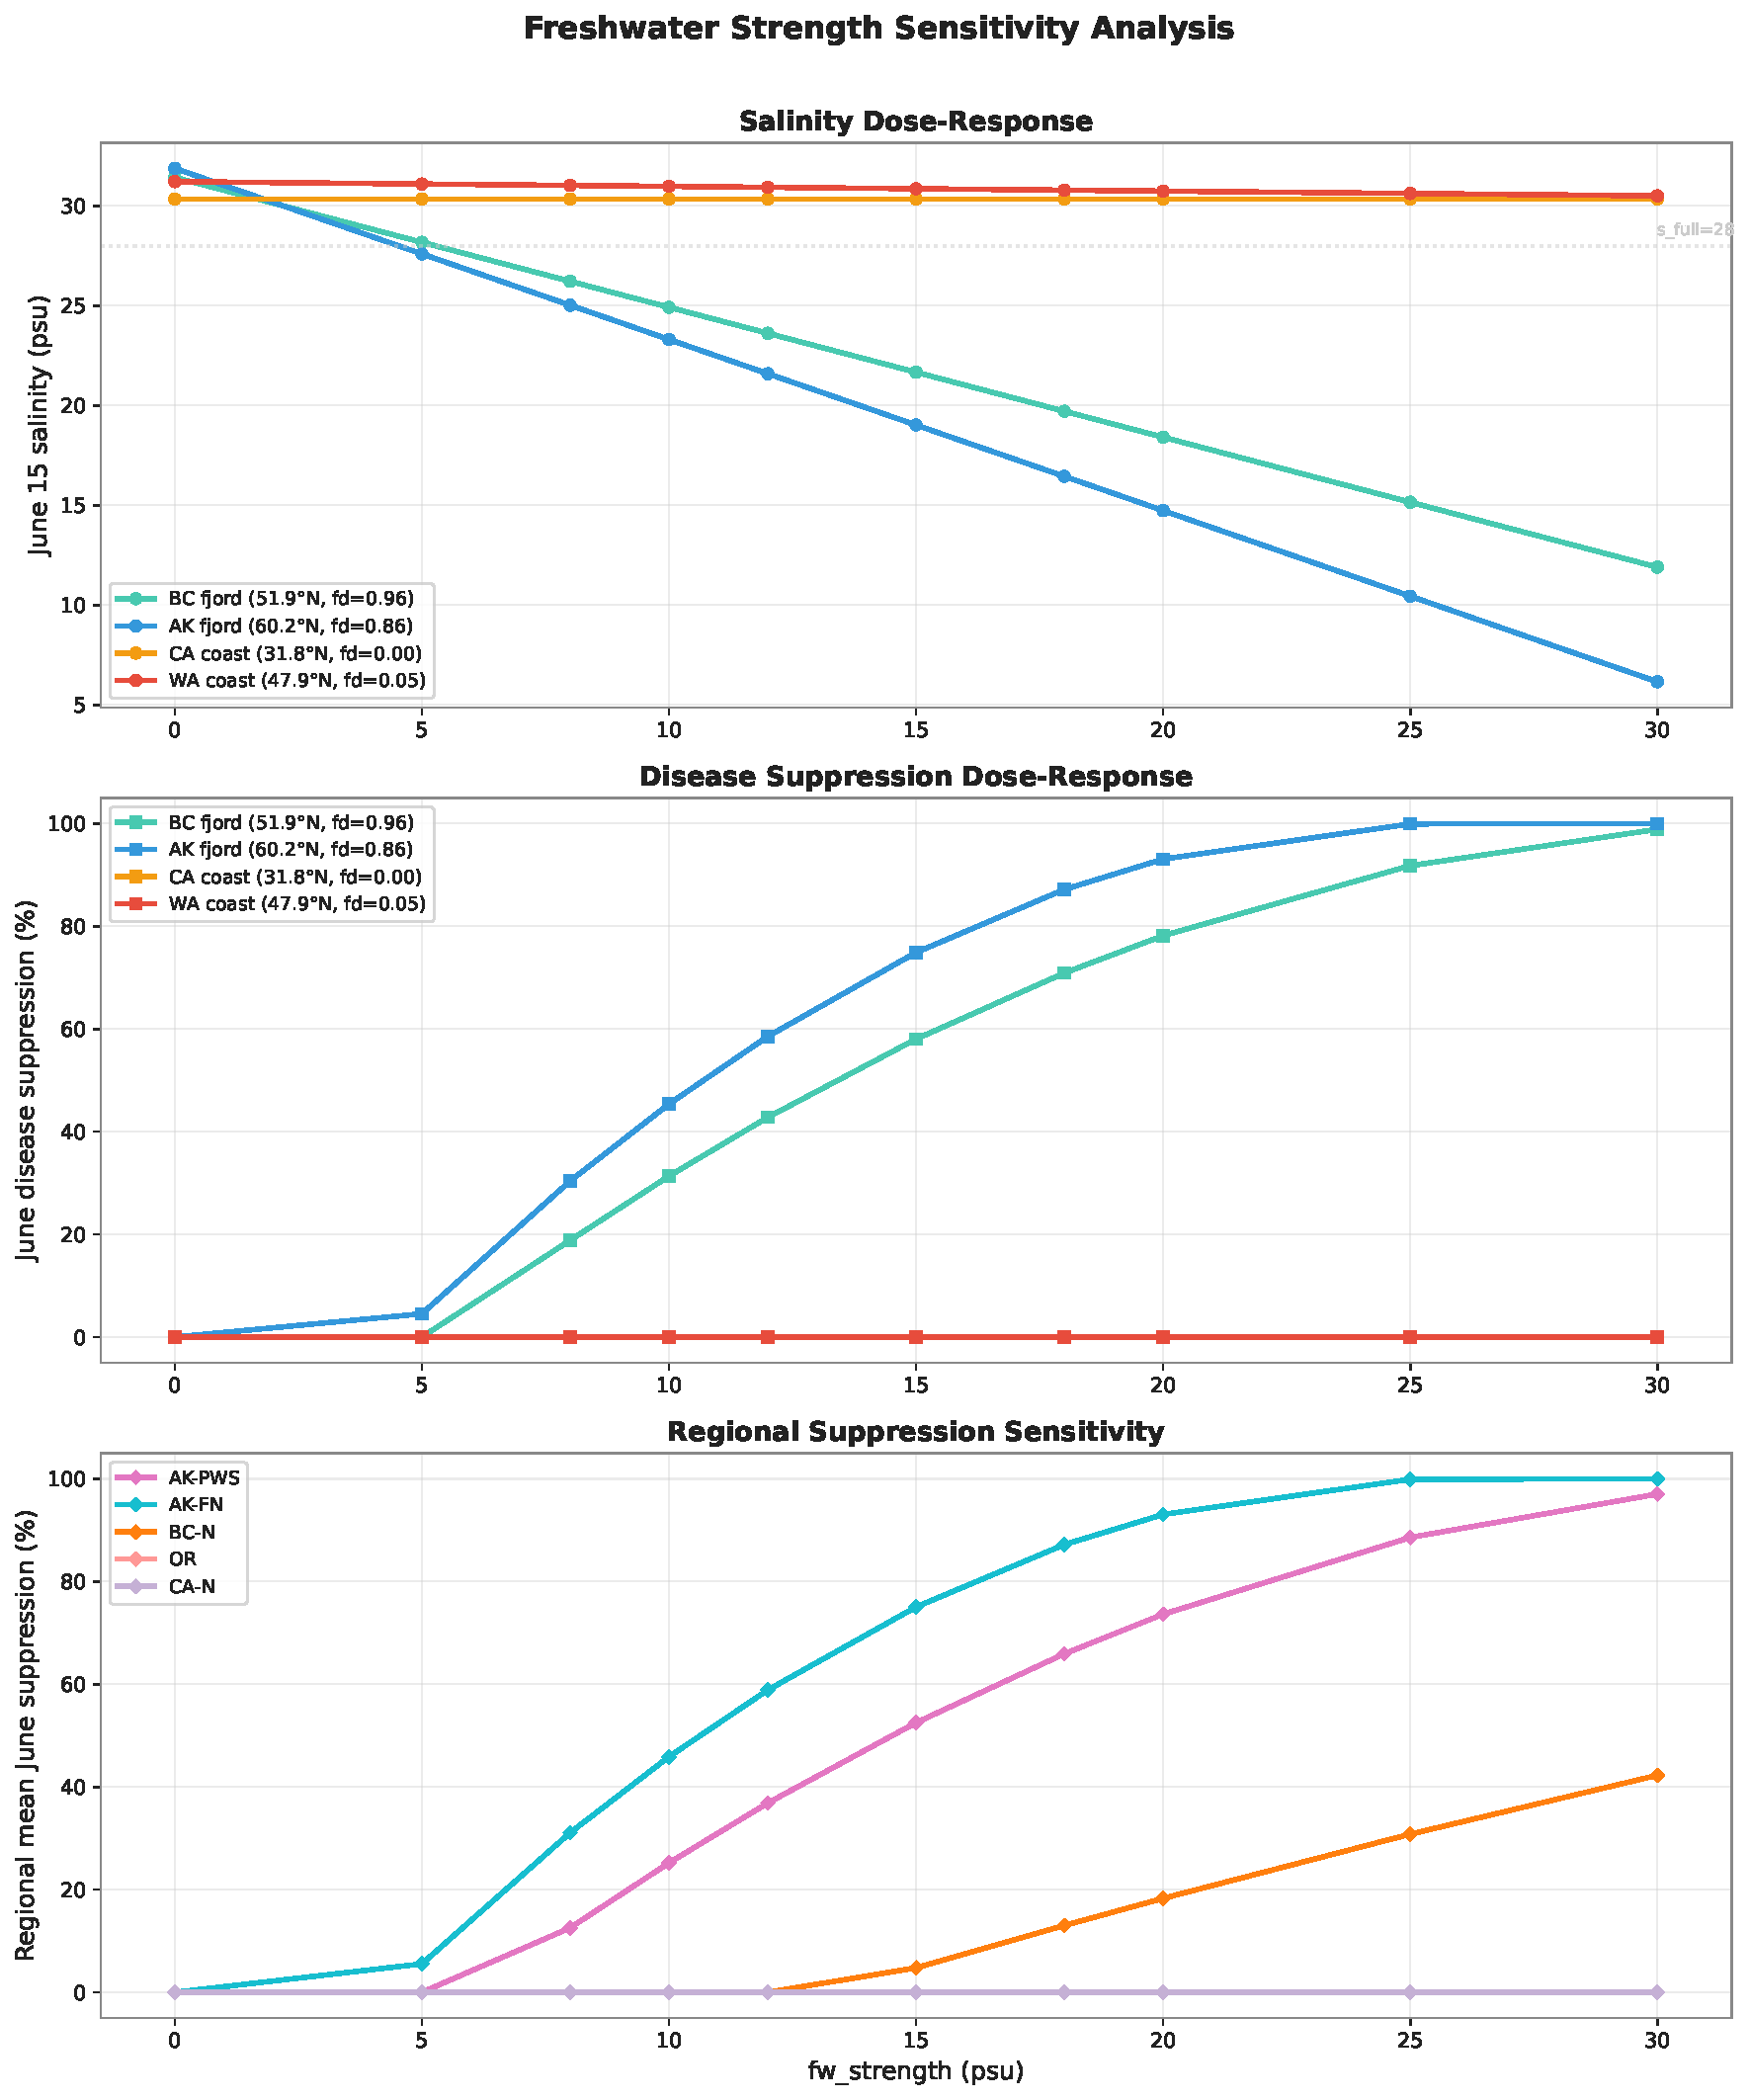
\includegraphics[width=0.95\textwidth]{fig_sensitivity.pdf}
\caption{Three-panel dose-response for \texttt{fw\_strength}. Left: mean June salinity vs.\ \texttt{fw\_strength} for selected regions. Center: mean June suppression (\%). Right: fraction of nodes experiencing $>$50\% suppression. The non-linear response through the $\texttt{sal\_mod}$ transfer function means suppression onset is abrupt once salinity drops below $\sim$22 psu.}
\label{fig:sensitivity}
\end{figure}

The dose-response is highly non-linear due to the $\eta = 2$ curvature in the $\texttt{sal\_mod}$ function. Moderate values of \texttt{fw\_strength} (6--10) produce detectable salinity depression but limited suppression (the depression keeps salinity above the 28 psu $s_{\text{full}}$ threshold at most sites). Higher values (15--20) push fjord sites below the steep part of the $\texttt{sal\_mod}$ curve, producing dramatic suppression. This threshold behavior means the data should provide relatively sharp constraints on \texttt{fw\_strength} during calibration.

\subsection{fw\_depth\_exp Sensitivity}

The \texttt{fw\_depth\_exp} parameter (range 0.3--3.0, default 1.0) controls how the fjord depth normalization maps to freshwater influence. Figure~\ref{fig:depth_exp} illustrates the effect of different exponent choices.

\begin{figure}[H]
\centering
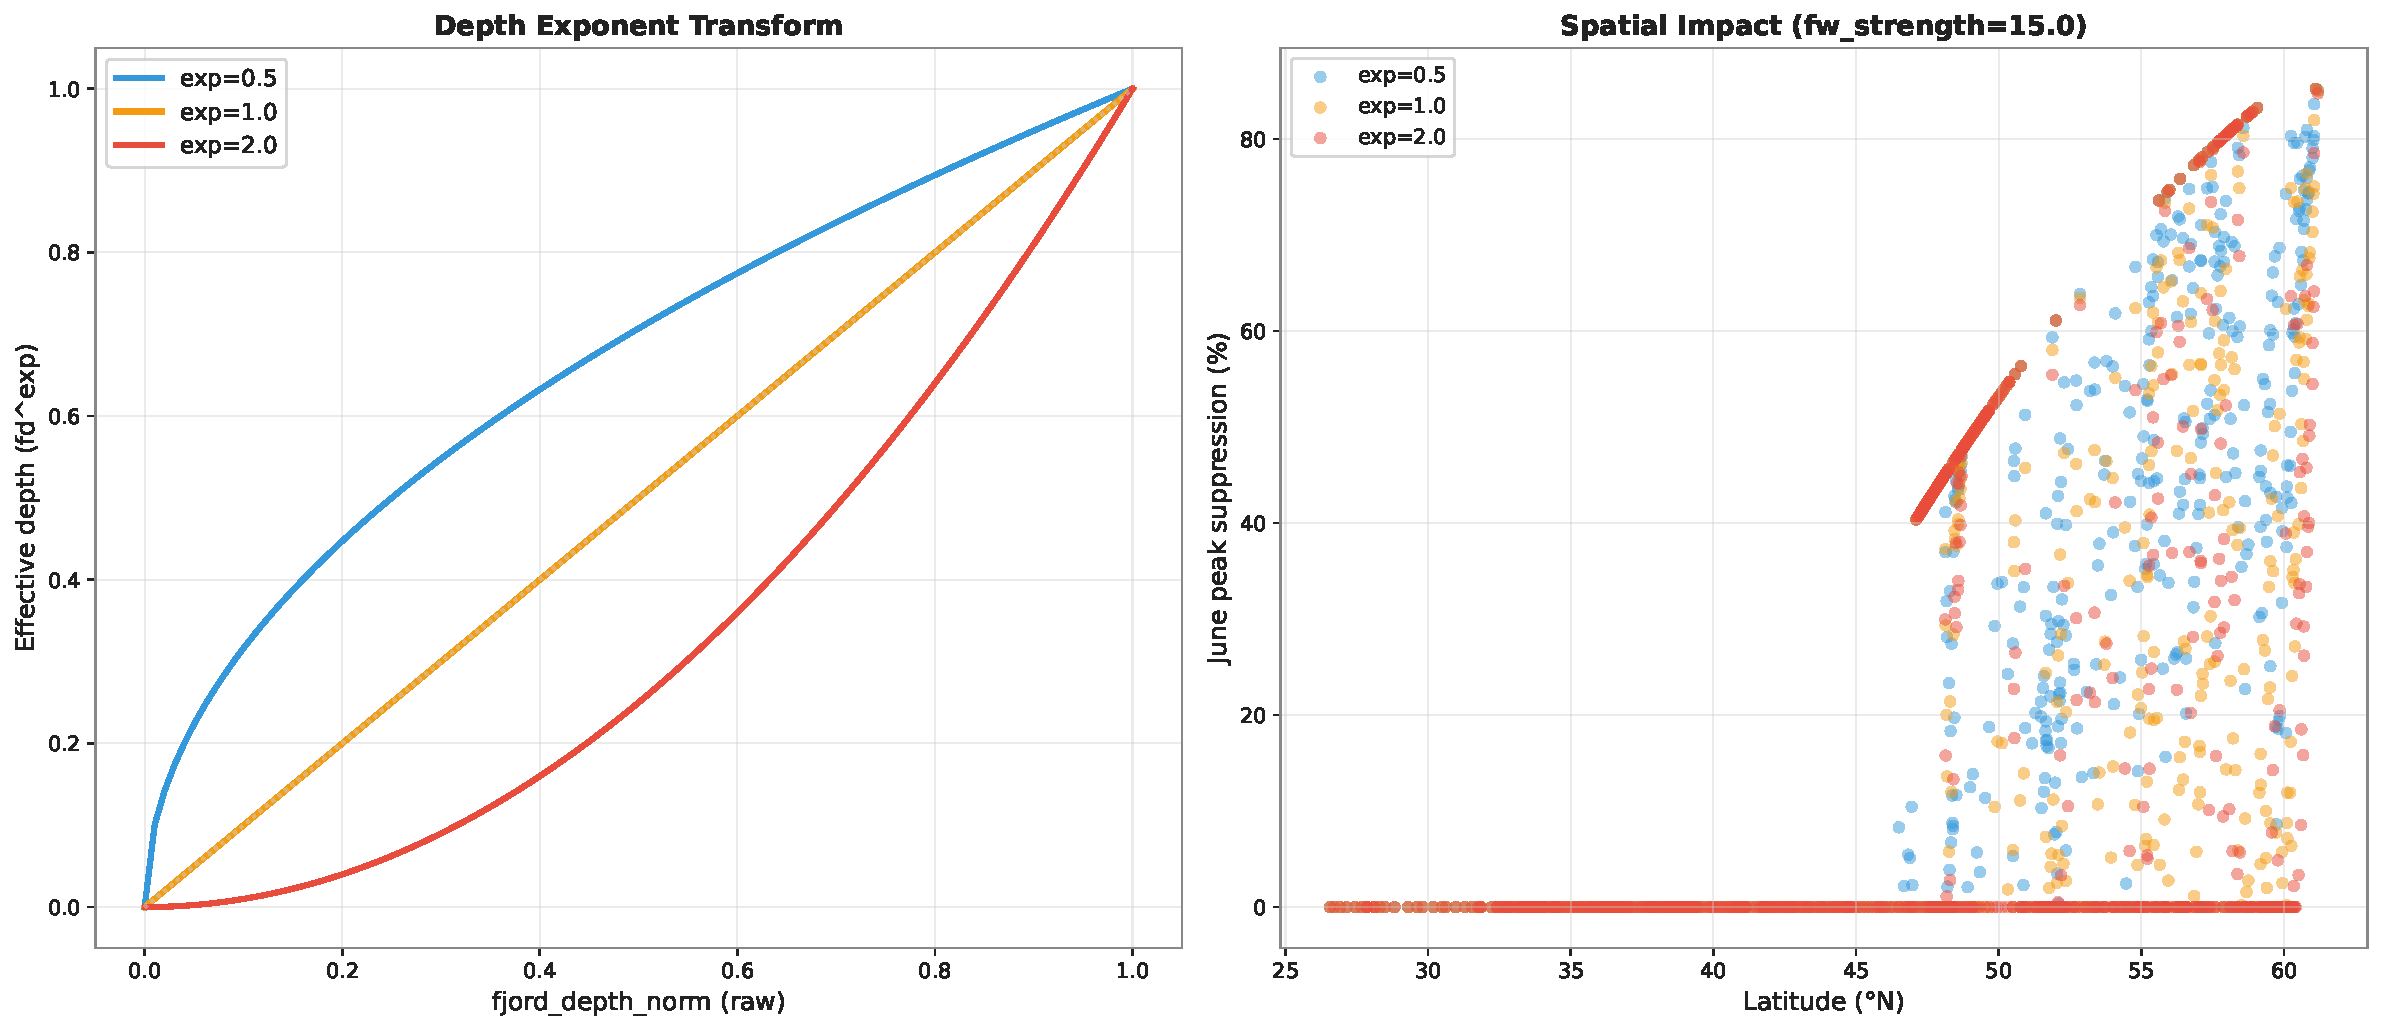
\includegraphics[width=0.85\textwidth]{fig_depth_exp.pdf}
\caption{Effect of \texttt{fw\_depth\_exp} on the fjord depth response. Three panels compare $\texttt{fd\_norm}^{0.5}$ (square root: broad effect, many sites affected), $\texttt{fd\_norm}^{1.0}$ (linear: default), and $\texttt{fd\_norm}^{2.0}$ (square: concentrated effect, only deepest fjords). Lower exponents spread the freshwater influence to more sites; higher exponents concentrate it in the most enclosed locations.}
\label{fig:depth_exp}
\end{figure}

\begin{itemize}
    \item $\texttt{fw\_depth\_exp} = 0.5$ (square root): Spreads freshwater effect broadly; even sites with $\texttt{fd\_norm} = 0.25$ retain 50\% of maximum depression. More nodes affected, shallower gradient.
    \item $\texttt{fw\_depth\_exp} = 1.0$ (linear): Default; depression scales proportionally with fjord depth.
    \item $\texttt{fw\_depth\_exp} = 2.0$ (square): Concentrates effect in deepest fjords; sites with $\texttt{fd\_norm} = 0.5$ experience only 25\% of maximum depression. Fewer nodes affected, steeper gradient.
\end{itemize}

The choice of exponent interacts with \texttt{fw\_strength}: a high exponent with high strength can produce similar network-wide patterns to a low exponent with moderate strength, creating a potential identifiability challenge in calibration.

% ============================================================
\section{Validation Against DFO Data}
\label{sec:validation}
% ============================================================

The 8 DFO lighthouse stations (Table~\ref{tab:dfo}) provide the only systematic ground-truth for the salinity model in the study region. Key validation findings:

\begin{enumerate}
    \item \textbf{Seasonal cycle captured:} All 8 stations show the expected winter-high, summer-low pattern. The model's cosine melt pulse reproduces this qualitative pattern, though the observed seasonality shows some asymmetry (faster spring decline than fall recovery at some stations) not captured by the symmetric pulse.

    \item \textbf{Enclosedness gradient reproduced:} The two most enclosed stations---Departure Bay (seasonal range 6.0 psu) and Chrome Island (4.4 psu)---show substantially larger seasonal ranges than exposed stations like Langara Island (1.6 psu). This is consistent with the model's use of \texttt{fjord\_depth\_norm} to modulate freshwater influence.

    \item \textbf{Ocean baseline bias:} The model baseline $S_{\text{ocean}}$ systematically exceeds observed winter (January) salinities by 0.2--1.8 psu, with the largest bias at Departure Bay (model: 31.28 psu, observed January: 29.5 psu). This reflects the fact that even winter salinity at enclosed sites is below true oceanic values.

    \item \textbf{Magnitude calibration needed:} The match between model depression and observed seasonal range depends on the \texttt{fw\_strength} and \texttt{fjord\_depth\_norm} assigned to each station. The DFO stations are primarily exposed to semi-exposed coastal sites, not deep fjords, so they sample the low end of the \texttt{fjord\_depth\_norm} distribution. Full validation of the extreme fjord predictions (10--15 psu depression) requires data from Alaska's inner fjords.
\end{enumerate}

% ============================================================
\section{Implications for Calibration}
\label{sec:calibration}
% ============================================================

The salinity mechanism introduces two new parameters into the MCMC calibration framework. Several considerations guide their integration:

\begin{enumerate}
    \item \textbf{Prior specification:} We recommend a weakly informative prior for \texttt{fw\_strength} centered around 12--15 psu, based on the DFO seasonal ranges and the requirement that Alaskan fjord suppression be detectable. For \texttt{fw\_depth\_exp}, a prior centered on 1.0 (linear) with moderate spread (0.5--2.0 at 90\% CI) seems appropriate.

    \item \textbf{Identifiability:} The \texttt{fw\_strength}--\texttt{fw\_depth\_exp} interaction creates a banana-shaped posterior ridge. The MCMC sampler should be tested for adequate exploration of this degeneracy. The sharp threshold in the $\texttt{sal\_mod}$ function may help break the degeneracy by providing constraint from binary presence/absence of disease at specific sites.

    \item \textbf{Computational cost:} The salinity calculation adds minimal overhead (vectorized numpy operations across 896 nodes $\times$ 365 days). No impact on overall MCMC runtime is expected.

    \item \textbf{Diagnostic nodes:} AK-FN sites (mean suppression 73.7\%) and AK-EG sites (mean suppression 0.8\%) form a natural contrast pair at similar latitudes but different fjord depths. Disease observations from these regions, if available, would be highly diagnostic for \texttt{fw\_strength}.

    \item \textbf{Salish Sea predictions:} The model predicts substantial suppression in SS-N (51.6\%) and SS-S (44.2\%). If disease data from these well-studied regions are inconsistent with this level of suppression, it would argue for lower \texttt{fw\_strength} values or modifications to the \texttt{fjord\_depth\_norm} assignments in the Salish Sea.
\end{enumerate}

% ============================================================
\section{Limitations and Future Work}
\label{sec:limitations}
% ============================================================

\begin{enumerate}
    \item \textbf{Static fjord depth normalization:} The \texttt{fjord\_depth\_norm} values are time-invariant, derived from GIS-based geomorphology. In reality, freshwater influence varies with precipitation, snowpack, and glacier mass balance---all of which are changing under climate warming.

    \item \textbf{Symmetric melt pulse:} The cosine melt pulse (Eq.~\ref{eq:melt_pulse}) is symmetric around the peak day, but real melt seasons often show rapid spring onset and gradual fall recession. An asymmetric pulse (e.g., gamma-shaped) could improve fit to DFO data.

    \item \textbf{No interannual variability:} The model produces identical salinity cycles each year. For multi-year simulations, incorporating year-specific snowpack or river discharge data could improve realism.

    \item \textbf{Ocean baseline simplicity:} The linear latitude dependence of $S_{\text{ocean}}$ (Eq.~\ref{eq:salinity}) neglects known spatial structure such as the California Current upwelling zone and the Alaska Coastal Current. A spatially-explicit baseline from ocean reanalysis products could be substituted.

    \item \textbf{Limited validation data:} The 8 DFO stations are all in BC (48--54\textdegree N) and do not include deep Alaskan fjords where the model predicts the strongest effects. Validation against Alaskan datasets (e.g., USGS, NOAA buoys) is a priority.

    \item \textbf{Vibrio salinity response:} The $\texttt{sal\_mod}$ parameters ($s_{\text{min}} = 10$, $s_{\text{full}} = 28$, $\eta = 2$) are based on literature values for \textit{V.\ coralliilyticus} and related species. Species-specific or strain-specific variation could alter the effective suppression thresholds.

    \item \textbf{Direct vs.\ indirect effects:} Salinity may affect sea star wasting through pathways beyond \textit{Vibrio} suppression (e.g., direct osmotic stress, microbiome shifts, immune function). The current model captures only the \textit{Vibrio}-mediated pathway.
\end{enumerate}

\vspace{1.5em}
\noindent\rule{\textwidth}{0.4pt}

\vspace{0.5em}
\noindent\textit{Report prepared for the SSWD-EvoEpi project. Data analysis and model implementation completed March 13, 2026. All source code, figure generation scripts, and node-level data are available in the project repository.}

\end{document}
